\chapter*{习题}
\phantomsection
\addcontentsline{toc}{chapter}{习题}
\setcounter{exercisegroup}{1}
\edef\CurrentExerciseGroup{\arabic{exercisegroup}}
\section*{\texorpdfstring{\S\CurrentExerciseGroup}{第{\CurrentExerciseGroup}节}}
\phantomsection
\addcontentsline{toc}{section}{第{\CurrentExerciseGroup}节习题}

\begin{enumerate}
\def\labelenumi{\arabic{enumi})}
\item
  设 E 是由函数 \(x \mapsto g(x) = \int_{0}^{x} f(t) dt\) （定义在 R 的区间 \([0,1]\) 上）所组成的向量空间，其中 f 取遍 \([0,1]\) 上的受控函数。设 P 是属于 E 的递增函数所成的集。试证 P 是一个凸锥，满足 E = P - P，\(P \cap (-P) = \{0\}\) ，并且 E 赋以由关系 \(g - h \in P\) 所定义的序结构后是一个 Riesz 空间。
\item
  设 \(I \subset \mathbf{R}\) 是一个紧区间。试证 \(\mathbf{R}^I\) 中由多项式函数（实系数）在 \(I\) 上的限制所组成的子空间是一个有向序空间，但不是 Riesz 空间。
\item
  \begin{enumerate}
  \def\labelenumii{\alph{enumii})}
  \tightlist
  \item
    设 E 是一个 Riesz 空间，H 是 E 的一个线性子空间。若对 H 中任意一对元素 x, y，\(\sup(x,y)\) 都属于 H，则称 H 为一个余格子子空间。此事成立当且仅当关系 \(x \in H\) 蕴涵 \(|x| \in H\) 。
  \end{enumerate}
\end{enumerate}

\begin{enumerate}
\def\labelenumi{\alph{enumi})}
\setcounter{enumi}{1}
\tightlist
\item
  设 I 是 R 中的一个紧区间，H 是 \(R^{I}\) 中由一次多项式 \(t \mapsto \alpha t + \beta\) 在 I 上的限制所组成的子空间。试证 H 不是 \(R^{I}\) 的余格子子空间，但 H 是一个 Riesz 空间（关于由 \(R^{I}\) 的结构诱导的结构）。
\end{enumerate}

\begin{enumerate}
\def\labelenumi{\arabic{enumi})}
\setcounter{enumi}{3}
\item
  设 E 是一个 Riesz 空间，H 是 E 的一个线性子空间。若关系 \(x \in H\) 与 \(|y| \leqslant |x|\) 蕴涵 \(y \in H\) ，则称 H 是 E 的一个孤立子空间。在此情形，设 P 是 E/H 中这样的元素 \(\dot{x}\) 所成的集：至少存在一个元素 \(x \geqslant 0\) 属于类 \(\dot{x}\) 。试证 P 是 E/H 上某个序结构的元素 \(\geqslant 0\) 全体所成的集，该序结构与 E/H 的向量空间结构相容，且对此结构 E/H 是一个 Riesz 空间（参见 A, VI, §1, 习题 4）。
\item
  \begin{enumerate}
  \def\labelenumii{\alph{enumii})}
  \tightlist
  \item
    若每个 \(x \in E\) ，只要使得 nx（n 为整数 \(\geqslant 0\) ）所成的集上有界，就必然 \(\leqslant 0\) ，则称序向量空间 E 是阿基米德的（A, VI, §1, 习题 31）。试证这一条件等价于：过 0 的任一平面与 E 的元素 \(\geqslant 0\) 所成的凸锥 P 的交是一个闭角域。试证为使一个序向量空间是阿基米德的，必须且只须它同构于某个完全格序空间的一个子空间（参见 A, VI, §1, 习题 31）。
  \end{enumerate}
\end{enumerate}

\begin{enumerate}
\def\labelenumi{\alph{enumi})}
\setcounter{enumi}{1}
\tightlist
\item
  设 F 是实值函数的 Riesz 空间 \(\mathbf{R}^{\mathbf{R}}\) （这些函数定义在 \(\mathbf{R}\) 上），并设 H 是有界函数所成的子空间 \(\mathcal{B}(\mathbf{R})\) （这些函数定义在 \(\mathbf{R}\) 上）；H 是 F 的一个孤立子空间（习题 4）。试证 Riesz 空间 \(\mathrm{E} = \mathrm{F} / \mathrm{H}\) （习题 4）不是阿基米德的：更确切地说，试证对 E 的每个元素 \(x \geqslant 0\) ，存在 \(y \in \mathrm{E}\) ，使得 \(y \geqslant nx\) 对每个整数 \(n \geqslant 0\) 成立。
\end{enumerate}

\begin{enumerate}
\def\labelenumi{\arabic{enumi})}
\setcounter{enumi}{5}
\item
  设 E 是一个完全格序空间，V 是 E 的一个线性子空间。试证：为使 E 中存在 V 的一个补 W 使 E 是 V 与 W 的序直和，必须且只须 V 是一个带；这时 W 必然等同于 E 中与 V 的每个元素都互奇异的元素所成的带。
\item
  设 E 是一个完全格序空间，H 是 E 的一个孤立子空间（习题 4）。若 \(B_{1}\) 与 \(B_{2}\) 是 E 中两个互余的带，试证 H 是 \(H_{1}=H\cap B_{1}\) 与 \(H_{2}=H\cap B_{2}\) 的序直和，且 Riesz 空间 E/H 是 Riesz 空间 \(B_{1}/H_{1}\) 与 \(B_{2}/H_{2}\) 的序直和。
\item
  设 \((\mathbf{E}_{\iota})\) 是一族完全格序空间，E 是诸 \(E_{\iota}\) 的乘积空间（它是完全格序的）。试证：若 B 是 E 中的一个带，则 B 的每个投影 \(\mathrm{B}_{\iota} = \mathrm{pr}_{\iota}(\mathrm{B})\) 是 \(E_{\iota}\) 中的一个带，且 B 等同于诸 \(B_{\iota}\) 的乘积。由此推出一个集合 A 到 R 中的映射所成的空间 \(R^{A}\) 中诸带的确定。试证在 A 上有界实值函数所成的空间 \(\mathcal{B}(A)\) 中，每个带都是某个带在 \(\mathcal{B}(A)\) 上的迹，而该带位于 \(R^{A}\) 中。
\item
  设 E 是一个完全格序空间。若 \(\mathfrak{F}\) 中存在一个上有界（相应地，下有界、有界）的集合，则称 E 上的滤子 \(\mathfrak{F}\) 是上有界的（相应地，下有界的、有界的）。对上有界（相应地，下有界）的滤子 \(\mathfrak{F}\) ，\(\mathfrak{F}\) 的上极限（相应地，下极限），记作 lim sup \(\mathfrak{F}\) （相应地，lim inf \(\mathfrak{F}\) ），定义为 E 的元素 \(\inf_{\mathrm{X}}(\sup \mathrm{X})\) （相应地，\(\sup_{\mathrm{X}}(\inf \mathrm{X})\) ），其中 X 取遍
\end{enumerate}

\(\mathfrak{F}\) 中上有界（相应地，下有界）的集合所成的集。若 \(\mathfrak{F}\) 有界，则 \(\liminf\mathfrak{F} \leqslant \limsup\mathfrak{F}\) ；称 \(\mathfrak{F}\) 关于 E 的序结构有一个极限或收敛，如果 \(\limsup\mathfrak{F} = \liminf\mathfrak{F}\) ；这时这两个元素的公共值记作 \(\lim\mathfrak{F}\) ，并称 \(\mathfrak{F}\) 收敛于 E 的这个元素。若有界滤子有一个极限，则每个更细的滤子有相同的极限（关于序结构）。

\begin{enumerate}
\def\labelenumi{\alph{enumi})}
\tightlist
\item
  为使有界滤子 \(\mathfrak{F}\) 关于序结构有一个极限，必须且只须 \(\inf_{\mathbf{X}} (\sup \mathbf{X} - \inf \mathbf{X}) = 0\) ，其中 \(\mathbf{X}\) 取遍 \(\mathfrak{F}\) 中有界的集合（可以利用下述事实：若在 E 中 \((x_{\alpha})\) 与 \((y_{\alpha})\) 是两个有下界的递减族，具有同一个右有向的指标集，则
\end{enumerate}

\[
\inf (x _ {\alpha} + y _ {\alpha}) = \inf x _ {\alpha} + \inf y _ {\alpha};
\]

为证明此公式，只需注意 \(\inf (x_{\alpha} + y_{\alpha})\leqslant x_{\beta} + y_{\gamma}\) 对每一对指标 \(\beta ,\gamma)\) 成立。

\begin{enumerate}
\def\labelenumi{\alph{enumi})}
\setcounter{enumi}{1}
\item
  设 A 是被滤子 G 过滤的集合，f 是 A 到 E 中的一个映射；若 \(f(\mathfrak{G})\) 是 E 中一个有极限（关于序结构）的有界滤子的基，则称 f 关于 G、按 E 的序结构有一个极限。试证：若 A 是一个有向序集，且 f 是 A 到 E 中的递增映射并在 A 上有上界，则 f 关于 A 的截面滤子有一个极限，等于 \(\sup f(x)\) 。
\item
  设 \((\mathbf{E}_{\iota})\) 是一族完全格序空间，E 是诸 \(E_{\iota}\) 的乘积完全格序空间。为使 E 上的有界滤子 F 关于序结构收敛，必须且只须对每个 \(\iota\) ，以 \(\Pr_{\iota}(\mathfrak{F})\) 为基的滤子在 \(E_{\iota}\) 中收敛；若 \(a_{\iota}\) 是其极限，则 \(a = (a_{\iota})\) 是 F 的极限。
\end{enumerate}

¶ 10) a) 设 E 是一个完全格序空间；E 上存在一个拓扑 \(\mathcal{T}_0(E)\) ，它是 E 的诸拓扑 \(\mathcal{T}\) 中最细的，使得每个按序结构意义（习题 9）收敛的有界滤子 \(\mathfrak{F}\) 对 \(\mathcal{T}\) 收敛于同一极限。

设 E 与 F 是两个完全格序空间，f 是 E 到 F 中的一个映射，使得对 E 上每个关于序结构收敛的有界滤子 F，\(f(\mathfrak{F})\) 是 F 上一个有界滤子的基，且该滤子关于序结构收敛于 \(f(\lim \mathfrak{F})\) 。试证在这些条件下，f 对拓扑 \(\mathcal{T}_{0}(\mathrm{E})\) 与 \(\mathcal{T}_{0}(\mathrm{F})\) 连续。

\begin{enumerate}
\def\labelenumi{\alph{enumi})}
\setcounter{enumi}{1}
\item
  由 a) 推出拓扑 \(\mathcal{T}_{0}(\mathrm{E})\) 与 E 的向量空间结构相容，且映射 \(x \mapsto |x|\) 对此拓扑连续。证明 \(\mathcal{T}_{0}(\mathrm{E})\) 与 E 的序向量空间结构相容，并由此推出此拓扑是 Hausdorff 的。
\item
  给定任一无穷集 A，设 \(\mathrm{E} = \mathcal{B}(\mathrm{A})\) 是 A 上有界实值函数所成的完全格序空间。设 \(\Phi\) 是定义在 A 上的数值函数 \(\varphi\) （有限与否皆可）的全体，这些函数满足 \(\varphi(t) > 0\) （对一切 \(t \in A\) ），且对每个整数 n \textgreater{} 0，\(t \in A\) 中使 \(\varphi(t) \leqslant n\) 者所成的集是有限的。对每个函数 \(\varphi \in \Phi\) ，设 \(V_{\varphi}\) 为 \(x \in E\) 中满足 \(|x| \leqslant \varphi\) 者所成的集；试证诸集 \(V_{\varphi}\) 构成一个拓扑 \(\mathcal{T}_{1}(\mathrm{E})\) 的 0 的基本邻域系，该拓扑与 E 的序向量空间结构相容，且对此拓扑 E 是 Hausdorff 的和完备的。试证拓扑 \(\mathcal{T}_{0}(\mathrm{E})\) 细于 \(\mathcal{T}_{1}(\mathrm{E})\) ，但严格粗于 A 上的一致收敛拓扑（由范数 \(\|x\| = \sup_{t \in A} |x(t)|\) 定义）（考虑元素 \(1 - \varphi_{X}\) ，它属于 \(\mathcal{B}(\mathrm{A})\) ，
\end{enumerate}

其中 X 取遍 A 的有限子集所成的集，\(\varphi_{X}\) 是 X 的特征函数）。由此推出，为使 E 的一个子集（关于序结构）有界，必须且只须它对拓扑 \(\mathcal{T}_{0}(E)\) 有界 (TVS, III, §1, No. 2)。试证 E 上每个有界且对拓扑 \(\mathcal{T}_{0}(E)\) 收敛的滤子关于序结构收敛于同一极限。最后，试证 E 上存在对 \(\mathcal{T}_{0}(E)\) 收敛但不有界的滤子。

¶ 11) 设 E 是一个完全格序空间，\((x_{\iota})_{\iota \in I}\) 是 E 的元素的一个族。对 I 的每个有限子集 H，令 \(s_{H} = \sum_{\iota \in H} x_{\iota}\) ；族 \((x_{\iota})_{\iota \in I}\) 称为关于 E 的序结构

可和的，如果映射 \(\mathrm{H} \mapsto s_{\mathrm{H}}\) 关于这一序结构、关于 I 的有限子集所成的有向序集 \(\mathfrak{F}(\mathrm{I})\) 有一个极限；这时这个极限 \(s\) 称为族 \((x_{\iota})_{\iota \in \mathrm{I}}\) 的和，记作 \(\sum_{\iota \in \mathrm{I}} x_{\iota}\) 。

\begin{enumerate}
\def\labelenumi{\alph{enumi})}
\item
  为使族 \((x_{\iota})_{\iota \in I}\) 可和，必须且只须：\(1^{\circ}\) 对 I 的每个有限子集 H，当 K 取遍 I 中与 H 不相交的有限子集所成的集时，诸 \(|s_{K}|\) 所成的集在 E 中有一个上确界 \(r_{\mathrm{H}}\) ；\(2^{\circ} \inf_{\mathrm{H}} r_{\mathrm{H}} = 0\) 当 H 取遍 \(\mathfrak{F}(I)\) （利用习题 9 a））。
\item
  把交换拓扑群中可和族的诸性质（GT, III, §5, 命题 2、3 与 Th. 2）推广到关于 E 的序结构的可和族。
\item
  设 \((x_{\iota})_{\iota \in I}\) 是 E 的元素 \(\geqslant 0\) 的一个族；为使该族可和，必须且只须有限部分和 \(s_{\mathrm{H}}\) 所成的集上有界（利用习题 9 b））。若 \((x_{\iota})_{\iota \in I}\) 可和，且 \((y_{\iota})_{\iota \in I}\) 是满足 \(0 \leqslant y_{\iota} \leqslant x_{\iota}\) （对一切 \(\iota\) ）的元素的一个族，试证族 \((y_{\iota})\) 可和，且 \(\sum_{\iota \in I} y_{\iota} \leqslant \sum_{\iota \in I} x_{\iota}\) ，其中等号仅当 \(x_{\iota} = y_{\iota}\) 对一切 \(\iota \in I\) 成立时成立。
\item
  设 \((x_{\iota})\) 是 E 的元素的一个族；试证若族 \((|x_{\iota}|)\) 关于序结构可和，则族 \((x_{\iota})\) 也可和。
\end{enumerate}

\begin{enumerate}
\def\labelenumi{\arabic{enumi})}
\setcounter{enumi}{11}
\tightlist
\item
  设 \(\mathbf{E}\) 是一个完全格序空间。试证存在一个族 \((u_{\iota})\) ，其元素 \(> 0\) 属于 \(\mathbf{E}\) ，使得 \(u_{\iota}\) 与 \(u_{\kappa}\) 对每一对不同的指标 \(\iota, \kappa\) 都互奇异，且对每个 \(x > 0\) （在 \(\mathbf{E}\) 中）至少存在一个指标 \(\iota\) 使 \(\inf(x, u_{\iota}) > 0\) （利用 Zorn 引理）。由此推出，对每个 \(x \geqslant 0\) ，存在唯一的一个族 \((x_{\iota})\) ，由元素 \(\geqslant 0\) （属于 \(\mathbf{E}\) ）组成，使得对每个 \(\iota, x_{\iota}\) 属于带 \(B_{\iota}\) （由 \(u_{\iota}\) 生成），且 \(x = \sum_{\iota} x_{\iota}\) （按 \(\mathbf{E}\) 的序结构）。
\end{enumerate}

（取 \(x_{\iota}\) 为 \(x\) 在带 \(B_{\iota}\) 中的分量）。反之，每个上有界的族 \((x_{\iota})\) ，由 E 的元素 \(\geqslant 0\) 组成，若满足 \(x_{\iota} \in B_{\iota}\) （对一切 \(\iota\) ），则在 E 中可和（习题 11）。

¶ 13 a) 设 E 是一个完全格序空间。若 \(u \neq 0\) 是 E 的任意一个元素，试证由这样的 \(x \in E\) 所成的集：存在一个整数 \(n\) 使得 \(|x| \leqslant n|u|\) ；该集是 E 的一个线性子空间 \(C_u\) ，它是 E 的一个完全格序的且余格子的子空间（习题 3）。对每个 \(x \in C_u\) ，用 \(\|x\|\) 表示标量 \(\lambda > 0\) （满足 \(|x| \leqslant \lambda |u|\) ）的下确界；试证 \(\|x\|\) 是 \(C_u\) 上的一个范数（利用 E 是阿基米德的这一事实（习题 5）），赋以此范数的 \(C_u\) 是完备的，且 \(\|x\| = \sup(\|x^+\|, \|x^-\|)\) 。

\begin{enumerate}
\def\labelenumi{\alph{enumi})}
\setcounter{enumi}{1}
\item
  设 \(\mathcal{I}\) 是 \(u\) 在空间 \(\mathrm{C}_u\) 的诸带中的分量所成的集；试证 \(\mathcal{I}\) 是由元素 \(c\) （属于 \(\mathrm{C}_u\) ，满足 \(0 \leqslant c \leqslant u\) 且 \(\inf(c, u - c) = 0\) ）组成的集（利用 Riesz 定理）。试证 \(\mathcal{I}\) 在赋范空间 \(\mathrm{C}_u\) 中是闭的，且对于由 \(\mathrm{C}_u\) 的序关系诱导的序关系，\(\mathcal{I}\) 是一个完备布尔代数（S, III, §1, 习题 11 与 17；只需证明若 \((c_\iota)\) 是 \(\mathcal{I}\) 的元素的一个族，则 \(\sup_{\iota} c_\iota\) 属于 \(\mathcal{I}\) ）。
\item
  设 \(x\) 是 \(\mathbf{C}_u\) 的任意一个元素；对每个 \(\lambda \in \mathbf{R}\) ，设 \(c(\lambda)\) 是 \(u\) 在 \(\mathbf{C}_u\) 的由 \((\lambda u - x)^+\) 生成的带中的分量。试证若 \(\lambda \leqslant \mu\) ，则 \(c(\lambda) \leqslant c(\mu)\) ；\(c(\lambda) = 0\) 对 \(\lambda < -\|x\|\) ，而 \(c(\lambda) = u\) 对 \(\lambda > \|x\|\) 。试证若 \(c \in \mathcal{I}\) 满足 \(c \leqslant c(\lambda)\) ，则 \(x\) 在由 \(c\) 生成的带中的分量 \(\leqslant \lambda c\) （注意由 \(c(\lambda)\) 生成的带与由 \((\lambda u - x)^+\) 生成的带是相同的，且 \(\lambda u - x\) 在此带中的分量等于 \((\lambda u - x)^+\) 在此带中的分量；由此推出 \(x\) 在这同一个带中的分量 \(\leqslant \lambda c(\lambda)\) ）。类似地，试证若 \(c \in \mathcal{I}\) 满足 \(c \leqslant u - c(\lambda)\) ，则 \(x\) 在由 \(c\) 生成的带中的分量 \(\geqslant \lambda c\) 。
\item
  已知（GT, II, §4, 习题 12）存在一个序结构同构 \(c \mapsto \theta_c\) ，它把布尔代数 \(\mathcal{I}\) 映到由一个紧全不连通空间 S 中既开又闭的集合的特征函数所组成的布尔代数上。试证关系 \(\sum_{i} \lambda_i c_i = 0\) 蕴涵函数 \(\sum_{i} \lambda_i \theta_{c_i}\) 在 S 上为 0（利用分解引理）；由这一注记与 c) 推出，映射 \(c \mapsto \theta_{c}\) 可以延拓为一个同构 \(x \mapsto \theta_{x}\) ，它把赋范空间 \(C_{u}\) 映到 S 上连续实值函数所成的赋范空间 \(\mathcal{C}(\mathrm{S};\mathbf{R})\) 上，使得 \((\theta_{x})^{+} = \theta_{x^{+}}\) 。（借助 c)，试证对每个 \(x \in C_{u}\) 与每个 \(\varepsilon > 0\) ，存在实数的一个递增序列 \((\lambda_{i})_{0 \leqslant i \leqslant n}\) ，使得 \(\lambda_{i} - \lambda_{i-1} \leqslant \varepsilon\)
\end{enumerate}

且 \(0 \leqslant x - \sum_{i=1}^{n} \lambda_{i-1} (c(\lambda_{i-1}) - c(\lambda_i)) \leqslant \varepsilon u\) 。

\begin{enumerate}
\def\labelenumi{\alph{enumi})}
\setcounter{enumi}{4}
\item
  为使 S 有限，必须且只须 \(C_{u}\) 是有限维的；由此（借助习题 12）推出每个有限维完全格序空间都同构于一个乘积空间 \(R^{n}\) （参见 §2, 习题 7）。
\item
  试证 S 是一个极不连通空间 (GT, I, §11, 习题 21)（利用 \(\mathcal{I}\) 是完备布尔代数这一事实）。极不连通紧空间称为 Stone 空间。试证若 X 是一个 Stone 空间，则对 X 上每个下半连续数值函数 \(f\) ，上半连续正则化 \(g\) （由 \(f\) 经正则化而得，GT, IV, §6, No. 2）是连续的（对每个 \(a < g(x)\) ，试证 \(x\) 不可能属于这样的 \(y\) 所成的（开）集的闭包：\(g(y) < a\) ；办法是注意 \(f(z) \leqslant a\) 在此集闭包的一点 \(z\) 处成立）。由此推出 \(\mathcal{C}(\mathrm{X};\mathbf{R})\) 这时是一个完全格序空间。试证当 Stone 空间 X 无穷时，一个上有界的集在 \(\mathcal{C}(\mathrm{X};\mathbf{R})\) 中的上确界未必等于它的上包络（考虑 X 中一个非闭的开集）；不过这两个函数在一个贫集的余集上相等（考虑使它们的差 \(\geqslant 1/n\) 的点所成的集）。
\item
  设 X 是一个 Stone 空间；试证若 f 是一个有界实值函数，定义在 X 的一个无处稠密子集 M 的余集上且在 X - M 上连续，则 \(f\) 可以连续地延拓到整个 X（利用 \(\mathcal{C}(X; \mathbf{R})\) 是完全格序的这一事实）。由此推出，若记 \(\mathcal{Q}(X; \overline{\mathbf{R}})\) 为 X 上（有限与否皆可的）连续数值函数 \(f\) 中满足 \(f(+\infty)\) 与 \(f(-\infty)\) 在 X 中无处稠密者所成的集，则它是一个完全格序向量空间。
\item
  试证 E 中由 u 生成的带 \(B_{u}\) （作为序空间）同构于 \(\mathcal{Q}(\mathrm{X};\overline{\mathbf{R}})\) 的一个孤立子空间（习题 4）（把元素 \(f \geqslant 0\) ——它属于 \(\mathcal{Q}(\mathrm{X};\overline{\mathbf{R}})\) ——看作诸元素 \(\inf(f,n)\) 的上确界）。
\end{enumerate}

\begin{enumerate}
\def\labelenumi{\arabic{enumi})}
\setcounter{enumi}{13}
\tightlist
\item
  设 E 是一个 Riesz 空间，带有一个与 E 的序向量空间结构相容的 Hausdorff 拓扑。
\end{enumerate}

\begin{enumerate}
\def\labelenumi{\alph{enumi})}
\item
  设 K 是 E 的一个紧子集，H 是 K 的一个对关系 \(\leqslant\) 有向的子集；试证 H 的截面滤子 F 收敛。（先证属于 K 的 H 的上界所成的集 L 非空且紧，再证 F 的接触点所成的集含于 L，最后证不可能存在两个不同的接触点。）
\item
  由 \(a\) ) 推出：若在 \(\mathbf{E}\) 中每个区间 \([a,b]\) 都是紧的，则 \(\mathbf{E}\) 是完全格序的。
\end{enumerate}

\setcounter{exercisegroup}{2}
\edef\CurrentExerciseGroup{\arabic{exercisegroup}}
\section*{\texorpdfstring{\S\CurrentExerciseGroup}{第{\CurrentExerciseGroup}节}}
\phantomsection
\addcontentsline{toc}{section}{第{\CurrentExerciseGroup}节习题}

\begin{enumerate}
\def\labelenumi{\arabic{enumi})}
\tightlist
\item
  设 E 是一个 Riesz 空间，x 是 E 的一个 \textgreater0 的元素。若存在 E 上的一个相对有界线性形式 L，使得 \(L(x) \neq 0\) ，试证 nx（n 为整数 \textgreater0）所成的集在 E 中不可能是上有界的。特别地，试证在 §1 习题 5 b) 所定义的 Riesz 空间 E 上不存在任何相对有界线性形式。
\end{enumerate}

¶ 2) a) 设 L 是 Riesz 空间 E 上的一个正线性形式。考虑 E 的一个元素 a \textgreater{} 0 以及满足下列条件的正线性形式 \(M \leqslant L\) 所成的集：\(1^{\circ} M(x) = L(x)\) 对每个满足 \(0 \leqslant x \leqslant a\) 的 x 成立；\(2^{\circ} M(x) = 0\) 对每个与 a 互奇异的 \(x \geqslant 0\) 成立。试证这个正线性形式的集有一个最大元素 \(L_{a}\) ，且对每个 \(x \geqslant 0\) ，\(L_{a}(x) = \inf L(y)\) ，其中 y 取遍满足 \(0 \leqslant y \leqslant x\) 且 x - y 与 a 互奇异的一切元素所成的集。试证 \(L_{\lambda a} = L_{a}\) 对每个标量 \(\lambda > 0\) 成立，且若 a 与 b 互奇异，则 \(L_{a+b} \leqslant L_{a} + L_{b}\) 。若 E 是完全格序的，试证当 a 与 b 在 E 中互奇异时 \(L_{a+b} = L_{a} + L_{b}\) 。

\begin{enumerate}
\def\labelenumi{\alph{enumi})}
\setcounter{enumi}{1}
\tightlist
\item
  取 E 为区间 \(\mathbf{I} = [0,1]\) （属于 \(\mathbf{R}\) ）上连续实值函数所成的 Riesz 空间，并取 \(L(x) = x\left(\frac{1}{2}\right)\) ；试用一个例子证明可以有 \(L_{a + b} < L_a + L_b\) ，对两个互奇异元素 \(a, b\) （属于 \(\mathbf{E}\) ）而言。
\end{enumerate}

\begin{enumerate}
\def\labelenumi{\arabic{enumi})}
\setcounter{enumi}{2}
\tightlist
\item
  设 \(\mathbf{E}\) 是一个完全格序空间。
\end{enumerate}

\begin{enumerate}
\def\labelenumi{\alph{enumi})}
\item
  试证：若线性形式 \(L\) 在 \(\mathbf{E}\) 上对拓扑 \(\mathcal{T}_0(\mathbf{E})\) （§1, 习题 10）连续，则它相对有界，且 \(|L|\) 对 \(\mathcal{T}_0(\mathbf{E})\) 连续（用反证法，注意对每个 \(x \in \mathbf{E}\) ，元素序列 \(x / n\) 当 \(n\) 趋于无穷时对拓扑 \(\mathcal{T}_0(\mathbf{E})\) 趋于 0）。
\item
  设 A 是任一无穷集，U 是 A 上的一个超滤子，其诸集合的交为空。在完全格序空间 \(E = \mathcal{B}(A)\) 上，考虑正线性形式 \(x \mapsto \lim_{\mu} x(t)\) ；试证此线性形式对拓扑 \(\mathcal{T}_{0}(E)\) 不连续。
\end{enumerate}

\begin{enumerate}
\def\labelenumi{\arabic{enumi})}
\setcounter{enumi}{3}
\tightlist
\item
  设 E 是一个完全格序空间。
\end{enumerate}

\begin{enumerate}
\def\labelenumi{\alph{enumi})}
\item
  设 \(L\) 是 \(\mathbf{E}\) 上的一个正线性形式，对拓扑 \(\mathcal{T}_0(\mathbf{E})\) （§1, 习题 10）连续。试证由 \(x \in \mathbf{E}\) （满足 \(L(|x|) = 0\) ）组成的集是一个带 \(Z(L)\) 。设 \(S(L)\) 为与 \(Z(L)\) 在 \(\mathbf{E}\) 中互余的带（§1, 习题 6）。
\item
  设 L 与 M 是 E 上两个正线性形式，对 \(\mathcal{T}_{0}(\mathrm{E})\) 连续。为使 M 属于 E 上相对有界线性形式所成的空间 \(\Omega\) 中由 L 生成的带，必须且只须 \(S(M) \subset S(L)\) 。（为看出条件是充分的，用反证法，假设 M 不满足命题 5 的条件；考虑 E 的元素的一个序列 \((y_{n})\) ，满足 \(0 \leqslant y_{n} \leqslant x\) ，
\end{enumerate}

\(L(y_{n}) \leqslant 1 / 2^{n}\) 且 \(M(y_{n}) \geqslant \alpha > 0\) ，并由此推出存在 E 的一个元素 \(z \geqslant 0\) ，使得 \(L(z) = 0\) 且 \(M(z) \geqslant \alpha\) 。

\begin{enumerate}
\def\labelenumi{\alph{enumi})}
\setcounter{enumi}{2}
\tightlist
\item
  设 \(L\) 与 \(M\) 是 \(\mathbf{E}\) 上两个正线性形式，对 \(\mathcal{T}_0(\mathbf{E})\) 连续。为使在 \(\Omega\) 中 \(L\) 与 \(M\) 互奇异，必须且只须 \(S(L) \cap S(M) = \{0\}\) 。（为看出条件是必要的，试证若 \(S(L) \cap S(M)\) 不化为 0，则 \(\Omega\) 中由 \(L\) 与 \(M\) 生成的带有公共元素 \(\neq 0\) ，办法是利用 b）。）
\end{enumerate}

¶ 5) a) 设 E 是一个 Riesz 空间，H 是 E 的一个孤立线性子空间（§1, 习题 4）。设 Ω 是 E 上相对有界线性形式所成的空间，设 Θ 是 Ω 中由在 H 上为零的线性形式 \(L \in \Omega\) 组成的子空间。试证 Θ 是 Ω 的一个孤立子空间，且 Θ 是一个完全格序空间，同构于 Riesz 空间 E/H 上相对有界线性形式所成的空间。

\begin{enumerate}
\def\labelenumi{\alph{enumi})}
\setcounter{enumi}{1}
\tightlist
\item
  设 \(u\) 是 \(E\) 到一个 Riesz 空间 \(F\) 中的线性映射；下列条件等价：
\end{enumerate}

\(\alpha) u(\sup(x, y)) = \sup(u(x), u(y));\)

\(\beta) u(\inf(x, y)) = \inf(u(x), u(y));\)

\(\gamma) u(x^{+}) = (u(x))^{+}\) ;

\(\delta)\) 关系 \(\inf (x,y) = 0\) 蕴涵 \(\inf (u(x),u(y)) = 0\)

这时称 u 是一个格线性映射。

\begin{enumerate}
\def\labelenumi{\alph{enumi})}
\setcounter{enumi}{2}
\item
  为使 E 的一个线性子空间 H 在孤立子空间 \(\neq\) E 的集合中是极大的，必须且只须它形如 \(\operatorname{Ker}(f)\) ，其中 \(f\) 是一个格线性形式 \(\neq 0\) 。（利用 GT, V, §3, 习题 1。）
\item
  给出一个不化为 0 且不含任何极大孤立子空间的 Riesz 空间的例子（参见 §1, 习题 5 b)）。
\end{enumerate}

¶ 6) 设 E 是一个 Riesz 空间，Ω 是 E 上相对有界线性形式所成的完全格序空间，F 是 Ω 的一个余格子子空间（§1, 习题 3）。对每个 \(x \in E\) ，映射 \(x' \mapsto \langle x, x' \rangle\) （由 F 到 R 中）是 F 上的一个相对有界线性形式 \(u_x\) ，且映射 \(x \mapsto u_x\) 是 E 到 F 上相对有界线性形式所成的完全格序空间 Ω' 中的一个递增线性映射。为使 \(x \mapsto u_x\) 是 E 到 Ω' 的一个余格子子空间上的同构，也就是说，为使 \(u_x > 0\) 蕴涵 x \textgreater{} 0，且 \(u_{\text{sup}(x,y)} = \text{sup}(u_x, u_y)\) ，必须且只须下列两个条件成立：1° 对 E 中每个 x \textgreater{} 0，存在 F 中的 \(x' > 0\) 使 \(\langle x, x' \rangle > 0\) ；2° 对 E 的每对互奇异元素 \(y \geqslant 0\) ， \(z \geqslant 0\) ，对每个数 \(\varepsilon > 0\) 以及 F 中每个 \(x' \geqslant 0\) ，存在 F 的两个元素 \(y' \geqslant 0\) ， \(z' \geqslant 0\) ，使得 \(x' = y' + z'\) 且 \(\langle y, y' \rangle + \langle z, z' \rangle \leqslant \varepsilon\) 。（注意：若第二个条件成立且 v 是 F 上的一个正线性形式，满足 \(v \geqslant u_x\) ，则有 \(v(x') \geqslant \langle x^+, x' \rangle - \varepsilon\) ，对 F 中每个 \(x' \geqslant 0\) 及每个 \(\varepsilon > 0\) 。）

若条件 \(2^{\circ}\) 成立而条件 \(1^{\circ}\) 不成立，则由元素 \(x \in E\) （满足 \(\langle x, x' \rangle = 0\) ，对一切 \(x' \in F\) ）组成的集是孤立线性子空间 \(H\) （在 \(E\) 中）。通过过渡到商，映射 \(x \mapsto u_x\) 这时定义 Riesz 空间 \(E / H\) 到 \(\Omega'\) 的一个余格子子空间上的一个同构。

试证当 \(\mathbf{F} = \Omega\) 时，上述条件 \(2^{\circ}\) 总成立（利用习题 2）。

\begin{enumerate}
\def\labelenumi{\arabic{enumi})}
\setcounter{enumi}{6}
\tightlist
\item
  设 \(E\) 是一个维数 \(n\) 有限的 Riesz 空间。
\end{enumerate}

\begin{enumerate}
\def\labelenumi{\alph{enumi})}
\item
  若 E 是阿基米德的（§1, 习题 5），试证 E 的元素 \(\geqslant 0\) 所成的锥 P 是闭的且有内点。由此推出 P 的诸支撑超平面的交化为 0（利用 \(P \cap (-P) = \{0\}\) 这一事实）。
\item
  利用 a) 与习题 6，试证每个维数 n 的阿基米德 Riesz 空间都同构于乘积空间 \(R^{n}\) （参见 §1, 习题 13 e)）。
\item
  给出一个维数 2 的全序 Riesz 空间的例子。
\end{enumerate}

¶ 8) 设 E 是一个 Riesz 空间，\((U_{\iota})\) 是 E 上正线性形式的一个族。我们考虑 E 上的拓扑 \(\mathcal{T}\) ，它由半范数 \(U_{\iota}(|x|)\) 定义。

\begin{enumerate}
\def\labelenumi{\alph{enumi})}
\item
  试证 E 中由满足 \(U_{\iota}(|x|)=0\) （对一切 \(\iota\) ）的 x 组成的子空间 H 是 E 的一个孤立子空间（§1, 习题 4）；E 相伴的 Hausdorff 空间是商空间 E/H；通过过渡到商，\(U_{\iota}\) 在 E/H 上定义正线性形式 \(\dot{U}_{\iota}\) ，且 E/H 上的商拓扑由半范数 \(\dot{U}_{\iota}(|\dot{x}|)\) 定义。
\item
  试证在空间 E 中映射 \(x \mapsto |x|\) 是一致连续的，并由此推出：若拓扑 T 是 Hausdorff 的，则它与 E 的序向量空间结构相容。
\item
  假设拓扑 \(\mathcal{T}\) 是 Hausdorff 的且 E 是完全格序的；试证 E 中每个带 B 都是闭的，且若 B' 是由与 B 的每个元素都互奇异的元素组成的带，则 E 是 B 与 B' 的拓扑直和。
\item
  假设拓扑 \(\mathcal{T}\) 是 Hausdorff 的。设 \(\overline{\mathrm{E}}\) 是 \(\mathrm{E}\) 的完备化；若 \(\mathrm{P}\) 是元素 \(\geqslant 0\) （属于 \(\mathrm{E}\) ）所成的集，试证 \(\overline{\mathrm{P}}\) （即 \(\mathrm{P}\) 在 \(\widehat{\mathrm{E}}\) 中的闭包）在 \(\widehat{\mathrm{E}}\) 上定义一个 Riesz 空间结构（参见 §1, No. 2）。
\item
  若 E 对拓扑 T 是 Hausdorff 的且完备的，试证为使一个集 \(A \subset E\) （按关系 \(\leqslant\) 有向）在 E 中有一个上确界，必须且只须对每个指标 \(\iota\) ，\(U_{\iota}(x)\) 在 A 中上有界；这时对 E 上每个连续的递增数值函数 f，有 \(\sup_{x \in A} f(x) = f(\sup A)\) 。由此
\end{enumerate}

推出 E 是完全格序的。

\begin{enumerate}
\def\labelenumi{\alph{enumi})}
\setcounter{enumi}{5}
\tightlist
\item
  假设 E 对拓扑 T 是 Hausdorff 的且完备的。试证若 E 上的滤子 F 关于 E 的序结构有一个极限（§1, 习题 9），则它对拓扑 T 收敛于同一极限（利用 e)）。
\end{enumerate}

\begin{enumerate}
\def\labelenumi{\arabic{enumi})}
\setcounter{enumi}{8}
\tightlist
\item
  设 E 是一个 Riesz 空间，\(\Omega\) 是 E 上相对有界线性形式所成的空间。考虑 \(\Omega\) 上由半范数 \(L \mapsto |L|(x)\) 定义的拓扑，其中 x 取遍 E 的元素 \(\geqslant 0\) 所成的集。试证赋以此拓扑的 \(\Omega\) 是 Hausdorff 的且完备的。
\end{enumerate}

\chapter{局部紧空间上的测度}

\section{局部紧空间上的测度}

\subsection{紧支集连续函数}

定义 1. --- 设 X 是一个拓扑空间，设 E 或者是 \(\overline{R}\) ，或者是 R 上的一个向量空间，并设 f 是 X 到 E 中的一个映射。X 中使 \(\mathbf{f}(x)=0\) 在 X-S 上成立的最小闭集 S （换句话说，一切 \(x\in X\) 中使 \(\mathbf{f}(x)\neq0\) 者所成的集在 X 中的闭包）称为 f 的支集，记作 Supp(f)。

设 X 是一个局部紧空间，E 是 R 或 C 上的一个拓扑向量空间；回忆一下，\(\mathcal{C}(X;E)\) 表示 X 到 E 中的连续映射所成的向量空间；当 E=R 或 E=C 时，若不致引起混淆，我们将省略此记号中的 E。我们将用 \(\mathcal{K}(X;E)\) 表示 \(\mathcal{C}(X;E)\) 中由具有紧支集的连续映射组成的子空间；对 X 的每个子集 A，我们用 \(\mathcal{C}(X,A;E)\) （相应地，\(\mathcal{K}(X,A;E)\) ）表示 \(\mathcal{C}(X;E)\) （相应地，\(\mathcal{K}(X;E)\) ）中由满足 Supp(f) ⊂ A 的映射 f 组成的子空间。若 E=R 或 E=C，在不致引起混淆时，我们写 \(\mathcal{K}(X)\) （相应地，\(\mathcal{K}(X,A)\) ）以代替 \(\mathcal{K}(X;\mathbf{R})\) 或 \(\mathcal{K}(X;\mathbf{C})\) （相应地，\(\mathcal{K}(X,A;\mathbf{R})\) 或 \(\mathcal{K}(X,A;\mathbf{C})\) ）；我们用 \(\mathcal{K}_{+}(X)\) 表示由函数 \(\geqslant0\) （属于 \(\mathcal{K}(X;\mathbf{R})\) ）组成的带顶点的凸锥。

对 X 的每个紧子集 K，空间 \(\mathcal{K}(X,K;E)\) 可以等同于连续函数空间 \(\mathcal{C}(K;E)\) 的一个子空间（即 K 到 E 中的连续映射中在 K 的边界 \(^{1}\) 上为零的那些所成的子空间）。当 \(\mathcal{C}(K;E)\) 赋以 K 中的一致收敛拓扑时，\(\mathcal{K}(X,K;E)\) 是 \(\mathcal{C}(K;E)\) 的一个闭子空间。特别地，若 E 是一个 Fréchet 空间（相应地，Banach 空间），则 \(\mathcal{K}(X,K;E)\) 亦然，因为若 E 的拓扑由半范数 \(p_{n}\) （相应地，范数 \(x \mapsto \|x\|\) ）定义，则 \(\mathcal{K}(X,K;E)\) 的拓扑由半范数 \(\mathbf{f} \mapsto \sup_{x \in K} p_n(\mathbf{f}(x))\) （相应地，范数 \(\mathbf{f} \mapsto \sup_{x \in K} \| \mathbf{f}(x) \|\) ，记作 \(\| \mathbf{f} \|\) ）定义。

空间 \(\mathcal{K}(\mathrm{X};\mathrm{E})\) 是子空间 \(\mathcal{K}(\mathrm{X},\mathrm{K};\mathrm{E})\) 的递增有向族之并，其中 K 取遍 X 的紧子集所成的集；此外，若 \(K_{1}\subset K_{2}\) 是 X 的两个紧子集，则典范单射 \(\mathcal{K}(\mathrm{X},\mathrm{K}_{1};\mathrm{E})\to\mathcal{K}(\mathrm{X},\mathrm{K}_{2};\mathrm{E})\) 对上述拓扑是连续的。若 E 是局部凸的，于是可以在 \(\mathcal{K}(\mathrm{X};\mathrm{E})\) 上定义直接极限\(^{2}\)——即诸 \(\mathcal{K}(\mathrm{X},\mathrm{K};\mathrm{E})\) 的局部凸拓扑的直接极限——（TVS, II, §4, No. 4）；除非明确说明相反的情形，当我们把 \(\mathcal{K}(\mathrm{X};\mathrm{E})\) 看作拓扑向量空间时，所说的总就是这个拓扑。

命题 1. --- 设 X 是一个局部紧空间，E 是一个 Hausdorff 局部凸空间。

\begin{enumerate}
\def\labelenumi{(\roman{enumi})}
\item
  局部凸空间 \(\mathcal{K}(\mathrm{X};\mathrm{E})\) 是 Hausdorff 的。对每个紧子集 \(\mathbf{K}\)（属于 \(\mathbf{X}\)），\(\mathcal{K}(\mathrm{X},\mathrm{K};\mathrm{E})\) 上由 \(\mathcal{K}(\mathrm{X};\mathrm{E})\) 的拓扑诱导的拓扑是 \(\mathbf{K}\) 中的一致收敛拓扑，且子空间 \(\mathcal{K}(\mathrm{X},\mathrm{K};\mathrm{E})\) 中的每一个在 \(\mathcal{K}(\mathrm{X};\mathrm{E})\) 中都是闭的。
\item
  若 \(\mathbf{E}\) 是有限个局部凸空间 \(\mathbf{E}_i\) （ \(1 \leqslant i \leqslant n\) ）的乘积，则映射 \(f \mapsto (\mathrm{pr}_i \circ f)\) 是空间 \(\mathcal{K}(\mathbf{X};\mathbf{E})\) 到乘积空间 \(\prod_{1 \leqslant i \leqslant n} \mathcal{K}(\mathbf{X};\mathbf{E}_i)\) 上的一个同构。
\item
  若 \(\mathrm{X}\) 是局部紧空间的一个族 \((\mathrm{X}_{\lambda})_{\lambda \in \mathrm{L}}\) 之和，则映射 \(f \mapsto (f|\mathrm{X}_{\lambda})_{\lambda \in \mathrm{L}}\) 是空间 \(\mathcal{K}(\mathrm{X};\mathrm{E})\) 到族 \((\mathcal{K}(\mathrm{X}_{\lambda};\mathrm{E}))_{\lambda \in \mathrm{L}}\) 的拓扑直和空间上的一个同构。
\item
  注意，在 \(\mathcal{K}(\mathrm{X};\mathrm{E})\) 上，X 中的一致收敛拓扑与 \(\mathcal{K}(\mathrm{X};\mathrm{E})\) 的向量空间结构相容，因为对每个 \(f\in \mathcal{K}(\mathrm{X};\mathrm{E})\) （其支集（紧）为 S），集 \(f(\mathrm{X}) = f(\mathrm{S})\cup \{0\}\) 是紧的，从而在 E 中有界（TVS, III, §3, No. 1, 命题 1）。由于这一拓扑 \(\mathcal{T}_0\) 是局部凸的且在每个 \(\mathcal{K}(\mathrm{X},\mathrm{K};\mathrm{E})\) 上诱导 K 中的一致收敛拓扑，故直接极限拓扑 \(\mathcal{T}\) （ \(\mathcal{K}(\mathrm{X};\mathrm{E})\) 上的）亦然（TVS, II, §4, No. 4, 注）；此外，\(\mathcal{T}\) 细于 \(\mathcal{T}_0\) 且 \(\mathcal{T}_0\) 是 Hausdorff 的，因此 \(\mathcal{T}\) 是 Hausdorff 的。最后，设函数 \(f\in \mathcal{K}(\mathrm{X};\mathrm{E})\) 属于 \(\mathcal{K}(\mathrm{X},\mathrm{K};\mathrm{E})\) 的闭包；根据定义，存在 X 的紧子集 \(\mathrm{K}'\supset \mathrm{K}\) 使 \(f\in \mathcal{K}(\mathrm{X},\mathrm{K}';\mathrm{E})\) 。由前所述，\(f\) 属于 \(\mathcal{K}(\mathrm{X},\mathrm{K};\mathrm{E})\) 在空间 \(\mathcal{K}(\mathrm{X},\mathrm{K}';\mathrm{E})\) 中的闭包，因而属于 \(\mathcal{K}(\mathrm{X},\mathrm{K};\mathrm{E})\) 。
\item
  直接极限中连续性的判别准则（TVS, II, §4, No. 4, 命题 5）立即表明映射 \(f \mapsto (\mathrm{pr}_i \circ f)\) 是连续的，且逆映射亦然（对后者，只需注意：若对每个函数 \(f_i \in \mathcal{K}(\mathrm{X};\mathrm{E}_i)\) 用 \(f_i'\) 表示 X 到 E 中满足 \(\mathrm{pr}_i\circ f_i' = f_i\) 以及 \(\mathrm{pr}_j\circ f_i' = 0\) （对 \(j\neq i\) ）的映射，则映射 \(f_{i}\mapsto f_{i}^{\prime}\) 中的每一个都是连续的）。
\item
  每个紧子集 \(\mathbf{K}\) （属于 \(\mathbf{X}\) ）只与如下那些 \(\mathbf{X}_{\lambda}\) 相交：它们属于一个有限子族 \((\mathbf{X}_{\lambda})_{\lambda \in \mathbf{H}}\) （ \((\mathbf{X}_{\lambda})_{\lambda \in \mathbf{L}}\) 的），并且立即可以看出，若令 \(\mathrm{K}_{\lambda} = \mathrm{K} \cap \mathrm{X}_{\lambda}\) （对 \(\lambda \in \mathbf{H}\) ），则映射 \(f \mapsto (f|\mathrm{X}_{\lambda})_{\lambda \in \mathbf{H}}\) 是 \(\mathcal{K}(\mathrm{X},\mathrm{K};\mathrm{E})\) 到 \(\prod_{\lambda \in \mathbf{H}} \mathcal{K}(\mathrm{X}_{\lambda},\mathrm{K}_{\lambda};\mathrm{E})\) 上的一个同构。反之，对每个函数 \(f_{\lambda} \in \mathcal{K}(\mathrm{X}_{\lambda};\mathrm{E})\) ，设 \(f_{\lambda}^{\prime \prime}\) 是 \(\mathbf{X}\) 到 \(\mathbf{E}\) 中满足 \(f_{\lambda}^{\prime \prime}|\mathrm{X}_{\lambda} = f_{\lambda}\) 以及 \(f_{\lambda}^{\prime \prime}|\mathrm{X}_{\mu} = 0\) （对 \(\mu \neq \lambda\) ）的映射；立即可以看出，映射 \(f_{\lambda} \mapsto f_{\lambda}^{\prime \prime}\) （\(\mathcal{K}(\mathrm{X}_{\lambda};\mathrm{E})\) 到 \(\mathcal{K}(\mathrm{X};\mathrm{E})\) 中的）是连续的。断言 (iii) 由这些注记以及直接极限中连续性的判别准则（TVS, II, §4, No. 4, 命题 5）得出。
\end{enumerate}

命题 2. --- 设 X 是一个局部紧空间，E 是一个 Hausdorff 局部凸空间。

\begin{enumerate}
\def\labelenumi{(\roman{enumi})}
\item
  若 \(\mathbf{E}\) 是一个 Fréchet 空间，则空间 \(\mathcal{K}(\mathbf{X};\mathbf{E})\) 是桶式的。
\item
  若 X 是仿紧的，则对 \(\mathcal{K}(\mathrm{X};\mathrm{E})\) 中每个有界集 B，存在 X 的一个紧子集 K，使得 \(\mathrm{B}\subset \mathcal{K}(\mathrm{X},\mathrm{K};\mathrm{E})\) 。
\end{enumerate}

设 E 是一个 Fréchet 空间。这时，对 X 的每个紧子集 K，\(\mathcal{K}(X,K;E)\) 是一个 Fréchet 空间，从而是桶式的，而且已知桶式空间的直接极限是桶式的（TVS, III, §4, No. 1, 命题 3 的推论 3），由此得 (i)。

若 X 是仿紧的，则已知（GT, I, §9, No. 10, Th. 5）X 是无穷远处可数的局部紧空间的一个族 \((\mathrm{X}_{\lambda})_{\lambda \in \mathrm{L}}\) 之和；\(^{3}\)于是（命题 1, (iii)），\(\mathcal{K}(\mathrm{X};\mathrm{E})\) 是子空间族 \(\mathcal{K}(\mathrm{X}_{\lambda};\mathrm{E})\) （ \(\lambda \in L\) ）的拓扑直和。根据拓扑直和中有界集的刻画（TVS, III, §1, No. 4, 命题 5），\(\mathcal{K}(\mathrm{X};\mathrm{E})\) 中每个有界集都含于有限个子空间 \(\mathcal{K}(\mathrm{X}_{\lambda};\mathrm{E})\) 之和，故只需证明 \(\mathcal{K}(\mathrm{X}_{\lambda};\mathrm{E})\) 中每个有界集都含于某个子空间 \(\mathcal{K}(\mathrm{X}_{\lambda},\mathrm{K}_{\lambda};\mathrm{E})\) ，其中 \(K_{\lambda}\) 是 \(X_{\lambda}\) 中的紧集。于是问题化为 X 无穷远处可数的情形，换言之，X 是相对紧开集的一个序列 \(U_{n}\) 之并，满足 \(\overline{U}_{n} \subset U_{n+1}\) （GT, I, §9, No. 9, 命题 15）。但这时 \(\mathcal{K}(\mathrm{X};\mathrm{E})\) 是空间序列 \(\mathcal{K}(\mathrm{X},\overline{\mathrm{U}}_{n};\mathrm{E})\) 的严格直接极限，由此得断言 (ii)（TVS, III, §1, No. 4, 命题 6）。

我们将称 \(\mathcal{K}(X;E)\) 的一个子集 H 是严格紧的，如果它是紧的且存在 X 的一个紧子集 K 使得 \(H \subset \mathcal{K}(X,K;E)\) 。由命题 2 立即得出：若 X 是一个仿紧局部紧空间且 E 是 Hausdorff 的，则 \(\mathcal{K}(X;E)\) 中每个紧集都是严格紧的。可以给出局部紧空间 X（非仿紧）的例子，使得 \(\mathcal{K}(\mathrm{X};\mathbf{R})\) 中存在是紧的但非严格紧的集（习题 3 与 4）。

\pandocbounded{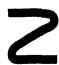
\includegraphics[keepaspectratio]{images/part001_73a6a0da.jpg}}

我们回忆，根据 Ascoli 定理（GT, X, §2, No. 5, Th. 2 的推论 3），\(\mathcal{K}(\mathrm{X};\mathrm{E})\) 的含于 \(\mathcal{K}(\mathrm{X},\mathrm{K};\mathrm{E})\) 中的严格紧子集 H 由下列条件刻画：\(1^{\circ}\) 它是闭的；\(2^{\circ}\) 它是等度连续的；\(3^{\circ}\) 对每个 \(x\in \mathbf{K}\) ，集 \(\mathrm{H}(x)\) 在 E 中相对紧。

推论. --- 设 X 是一个仿紧局部紧空间；若 E 是一个拟完备局部凸空间，则空间 \(\mathcal{K}(X;E)\) 是拟完备的。

根据命题 2, (ii)，只需注意：对 X 的每个紧子集 K，\(\mathcal{K}(X,K;E)\) 是 \(\mathcal{C}(K;E)\) 的一个闭子空间，后者是拟完备的，因为 \(\mathcal{C}(K;E)\) 的每个有界子集都由取值于 E 的同一个有界子集中的函数组成。

\subsection{逼近性质}

引理 1. --- 设 X 是一个局部紧空间，K 是 X 的一个紧子集，\((\mathrm{V}_{k})_{1\leqslant k\leqslant n}\) 是 K 由 X 的开集组成的一个有限覆盖。则存在 n 个连续映射 \(f_{k}\) （把 X 映到 {[}0,1{]} 中），使得 \(f_{k}\) 的支集含于 \(V_{k}\) （对 \(1\leqslant k\leqslant n\)），且 \(\sum_{k=1}^{n}f_{k}(x)\leqslant1\) 对所有 \(x\in X\) 成立，\(\sum_{k=1}^{n}f_{k}(x)=1\) 对所有 \(x\in K\) 成立。

因为，设 \(X'\) 是由 X 添加一个无穷远点 \(\omega\) 而得到的紧空间（GT, I, §9, No. 8, Th. 4）；诸集合 \(V_{0} = X' - K\) 与 \(V_{k}\) （ \(1 \leqslant k \leqslant n\) ）构成 \(X'\) 的一个开覆盖。设 \((f_{k})_{0 \leqslant k \leqslant n}\) 是从属于 \(X'\) 的这一覆盖的一个连续单位分解（GT, IX, §4, No. 3, 命题 3）；诸函数 \(f_{k}\) （指标 \(k \geqslant 1\) ）满足引理的条件。

引理 2. --- 设 X 是一个局部紧空间，K 是 X 的一个紧子集，E 是一个局部凸空间，q 是 E 上的一个连续半范数，\(\Phi\) 是 X 到 E 中的映射所成的一个等度连续集，其诸支集都含于 K。则对每个 \(\varepsilon > 0\) ，存在 X 上的一个连续单位分解 \((\varphi_{j})_{0 \leqslant j \leqslant n}\) ，具有下列性质：

\begin{enumerate}
\def\labelenumi{(\roman{enumi})}
\item
  \(\operatorname{Supp}(\varphi_j) \subset \mathrm{K}\) 对 \(1 \leqslant j \leqslant n\) 成立。
\item
  若对 \(1 \leqslant j \leqslant n\) ，\(x_j\) 是 \(\operatorname{Supp}(\varphi_j)\) 的任意一点，则对每个函数 \(\mathbf{f} \in \Phi\) 及每个 \(x \in \mathbf{X}\) ，
\end{enumerate}

\[
q \left(\mathbf {f} (x) - \sum_ {j = 1} ^ {n} \varphi_ {j} (x) \mathbf {f} \left(x _ {j}\right)\right) \leqslant \varepsilon .\tag{1}
\]

对属于 K 的边界的每个 \(y\) ，有 \(\mathbf{f}(y) = 0\) （对一切 \(\mathbf{f} \in \Phi\) ），因此存在一个开邻域 \(\mathrm{V}_y\) （\(y\) 在 X 中的），使得对每个 \(z \in \mathrm{V}_y\) 及每个 \(\mathbf{f} \in \Phi\) ，有 \(q(\mathbf{f}(z)) \leqslant \varepsilon / 2\) 。设 \(\mathrm{K}'\) 是 K 中不属于任何 \(\mathrm{V}_y\) （当 \(y\) 取遍 K 的边界）的点所成的集；\(\mathrm{K}'\) 是紧的且含于 K 的内部。集 \(\Phi\) 在 K 中是一致等度连续的；因此存在一个有限开覆盖 \((\mathrm{U}_j)_{1 \leqslant j \leqslant n}\) （\(\mathrm{K}'\) 的，由含于 K 的 X 的开集组成），使得对每对点 \(x, y\) （同一个 \(\mathrm{U}_j\) 中的），有 \(q(\mathbf{f}(x) - \mathbf{f}(y)) \leqslant \varepsilon / 2\) （对每个 \(\mathbf{f} \in \Phi\) ）。由引理 1，存在 \(n\) 个连续映射 \(\varphi_j\) （X 到 {[}0,1{]} 中的； \(1 \leqslant j \leqslant n\) ），使得 \(\operatorname{Supp}(\varphi_j) \subset \mathrm{U}_j\) ，且 \(\sum_{j=1}^{n} \varphi_j(x) \leqslant 1\) 在 X 上成立，\(\sum_{j=1}^{n} \varphi_j(x) = 1\) 在 \(\mathrm{K}'\) 上成立。对 \(x_j \in \operatorname{Supp}(\varphi_j)\) （ \(1 \leqslant j \leqslant n\) ）及 \(\mathbf{f} \in \Phi\) ，我们于是有：对一切 \(x \in \mathrm{U}_j\) ，

\[
q \big (\mathbf {f} (x) \varphi_ {j} (x) - \mathbf {f} (x _ {j}) \varphi_ {j} (x) \big) = \varphi_ {j} (x) q \big (\mathbf {f} (x) - \mathbf {f} (x _ {j}) \big) \leqslant \frac {\varepsilon}{2} \varphi_ {j} (x),
\]

且当 \(x \notin U_{j}\) 时这一关系仍成立，因为这时 \(\varphi_{j}(x) = 0\) 。相加即得：对每个 \(x \in X\) ，

\[
q \left(\mathbf {f} (x) \left(1 - \varphi_ {0} (x)\right) - \sum_ {j = 1} ^ {n} \varphi_ {j} (x) \mathbf {f} \left(x _ {j}\right)\right) \leqslant \frac {\varepsilon}{2} \left(1 - \varphi_ {0} (x)\right),\tag{2}
\]

其中 \(\varphi_0 = 1 - \sum_{j=1}^{n} \varphi_j\) ；由此当 \(x \in \mathbf{K}'\) 时得 (1)，因为这时 \(\varphi_0(x) = 0\) ；当 \(x \notin \mathbf{K}\) 时 (1) 也成立，因为这时第一项为零。最后，对 \(x \in \mathbf{K} - \mathbf{K}'\) ，有 \(q(\mathbf{f}(x)\varphi_0(x)) \leqslant \varepsilon/2\) （由 \(\mathbf{K}'\) 的定义），因此这一关系与 (2) 在此情形仍蕴涵 (1)。

设 X 是一个局部紧空间；对每个 Banach 空间 E（实的或复的），我们用 \(\mathcal{C}^{b}(X;E)\) 表示 X 到 E 中的连续且有界的映射所成的向量空间；已知 X 中的一致收敛拓扑与 \(\mathcal{C}^{b}(X;E)\) 的（实的，相应地，复的）向量空间结构相容，且它由范数

\[
\| \mathbf {f} \| = \sup _ {x \in X} \| \mathbf {f} (x) \|.\tag{3}
\]

此外，这样定义的赋范空间是一个 Banach 空间（GT, X, §3, No. 2, 以及 No. 1, 命题 2 的推论 2）；这一范数在 \(\mathcal{K}(\mathrm{X};\mathrm{E})\) 上定义的拓扑（换句话说，X 中的一致收敛拓扑）粗于第 1 目中在 \(\mathcal{K}(\mathrm{X};\mathrm{E})\) 上定义的直接极限拓扑。

命题 3. --- 设 X 是一个局部紧空间，X‘ 是由 X 添加一个无穷远点 ω 而得到的紧空间（GT, I, §9, No. 8,

Th. 4)，E 是一个 Banach 空间。\(\mathcal{K}(\mathrm{X};\mathrm{E})\) 在赋范空间 \(\mathcal{C}^b (\mathrm{X};\mathrm{E})\) 中的闭包是 \(\mathbf{X}\) 上以 E 为值且在点 \(\omega\) 处趋于 0 的连续函数所成的向量空间。

设 \(\mathbf{f} \in \mathcal{C}^b(\mathrm{X};\mathrm{E})\) 是属于 \(\mathcal{K}(\mathrm{X};\mathrm{E})\) 的闭包中的一个函数；对每个 \(\varepsilon > 0\) ，存在一个函数 \(\mathbf{g} \in \mathcal{K}(\mathrm{X};\mathrm{E})\) ，使得 \(\| \mathbf{f}(x) - \mathbf{g}(x) \| \leqslant \varepsilon\) 对所有 \(x \in \mathrm{X}\) 成立；若 \(\mathrm{K}\) 是 \(\mathbf{g}\) 的支集，则由此得出 \(\| \mathbf{f}(x) \| \leqslant \varepsilon\) 对所有 \(x \in \complement \mathrm{K}\) 成立，从而 \(\mathbf{f}(x)\) 当 \(x\) 趋于 \(\omega\) 时趋于 0。反之，若 \(\mathbf{f}\) 具有这一性质，则对每个 \(\varepsilon > 0\) ，存在一个紧集 \(\mathrm{K} \subset \mathrm{X}\) ，使得 \(\| \mathbf{f}(x) \| \leqslant \varepsilon\) 对所有 \(x \in \complement \mathrm{K}\) 成立。由引理 1，存在一个连续映射 \(h\) （X 到 {[}0,1{]} 中的），具有紧支集且在 \(\mathrm{K}\) 上等于 1；这时 \(\| \mathbf{f}(x) h(x) \| \leqslant \varepsilon\) 在 \(\complement \mathrm{K}\) 上成立，且 \(\mathbf{f}(x) = \mathbf{f}(x) h(x)\) 在 \(\mathrm{K}\) 上成立；由于 \(\mathbf{f}h\) 具有紧支集且 \(\| \mathbf{f}(x) - \mathbf{f}(x) h(x) \| \leqslant 2\varepsilon\) 对所有 \(x \in \mathrm{X}\) 成立，命题得证。

我们将用 \(\mathcal{C}^{0}(\mathrm{X};\mathrm{E})\) 表示 \(\mathcal{C}^{b}(\mathrm{X};\mathrm{E})\) 中由在无穷远点 \(\omega\) 处趋于零的函数组成的子空间；它也就是赋范空间 \(\mathcal{K}(\mathrm{X};\mathrm{E})\) 的完备化。

命题 4. --- 设 X 是一个局部紧空间，E 是一个局部凸空间；则空间 \(\mathcal{K}(\mathrm{X};\mathrm{E})\) 在 \(\mathcal{C}(\mathrm{X};\mathrm{E})\) 中对紧收敛拓扑是稠密的。

对每个紧集 \(K \subset X\) ，由引理 1，存在一个在 K 上等于 1 的函数 \(h \in \mathcal{K}(X; \mathbf{R})\) ；对每个函数 \(\mathbf{f} \in \mathcal{C}(X; E)\) ，函数 hf 属于 \(\mathcal{K}(X; E)\) 且在 K 上等于 f，由此得我们的断言。

命题 5. --- 设 X 是一个局部紧空间，E 是一个实的（相应地，复的）局部凸空间。对 X 的每个紧子集 K，向量空间 \(\mathcal{K}(X,K;\mathbf{R})\otimes_{\mathbf{R}}E\) （相应地，\(\mathcal{K}(X,K;\mathbf{C})\otimes_{\mathbf{C}}E\) ）（等同于 X 到 E 中的映射所成的一个集，参见 A, II, §7, No. 7, 命题 15 的推论）在 \(\mathcal{K}(X,K;E)\) 中稠密；向量空间 \(\mathcal{K}(X;\mathbf{R})\otimes_{\mathbf{R}}E\) （相应地，\(\mathcal{K}(X;\mathbf{C})\otimes_{\mathbf{C}}E\) ）在 \(\mathcal{K}(X;E)\) 中稠密。

由于第二个断言是第一个断言的明显推论，只需证明后者。我们应用引理 2，其中 \(\Phi\) 化为 \(\mathcal{K}(X,K;E)\) 的单个元素 f；这时，对每个 \(x\in X\) ，

\[
q \left(f (x) - \sum_ {j = 1} ^ {n} \varphi_ {j} (x) f \left(x _ {j}\right)\right) \leqslant \varepsilon ,
\]

其中 \(\varphi_{j}\) 属于 \(\mathcal{K}(\mathrm{X},\mathrm{K};\mathbf{R})\) ；由于映射 \(x\mapsto \sum_{j = 1}^{n}\varphi_{j}(x)f(x_{j})\) 可以典范地等同于元素 \(\sum_{j = 1}^{n}\varphi_{j}\otimes f(x_{j})\) ，由 \(\mathcal{K}(\mathrm{X},\mathrm{K};\mathrm{E})\) 的拓扑的定义，这就证明了命题。

\subsection{测度的定义}

定义 2. --- \(\mathcal{K}(\mathrm{X};\mathbf{C})\) （\(\mathrm{X}\) 为一个局部紧空间）上的一个连续线性形式称为 \(\mathrm{X}\) 上的一个测度（或复测度）。

若 \(\mu\) 是局部紧空间 \(X\) 上的一个测度，则测度对一个函数 \(f \in \mathcal{K}(X; \mathbf{C})\) 所取的值称为 \(f\) 关于 \(\mu\) 的积分；除了通用记号 \(\mu(f)\) 与 \(\langle f, \mu \rangle\) 之外，也使用记号 \(\int f d\mu, \int f\mu, \int f(x) d\mu(x)\) 与 \(\int f(x)\mu(x)\) 来表示它；关于字母 \(x\) 的用法，参见 S, I, §1, No. 1。

根据直接极限中连续性的判别法（TVS, Ch. II, §4, No. 4, 命题 5），说 \(\mu\) 是 X 上的一个测度，就是说 \(\mu\) 是 \(\mathcal{K}(\mathrm{X};\mathbf{C})\) 上满足下述条件的线性形式：对 X 的每个紧子集 K，存在一个数 \(\mathrm{M_K}\) ，使得对每个支集含于 K 的函数 \(f\in \mathcal{K}(\mathrm{X};\mathbf{C})\) ，

\[
| \mu (f) | \leqslant \mathrm{M} _ {\mathrm{K}} \cdot \| f \| \quad (\text { where } \| f \| = \sup _ {x \in \mathrm{X}} | f (x) |).\tag{4}
\]

更一般地：

命题 6. --- 设 X 是一个局部紧空间，\((\mathrm{K}_{\alpha})\) 是 X 的一族紧子集，它们的内部 \(\mathring{K}_{\alpha}\) 构成 X 的一个开覆盖。为使线性形式 \(\mu\) （\(\mathcal{K}(\mathrm{X};\mathbf{C})\) 上的）是 X 上的测度，必须且只须对每个 \(\alpha\) 存在一个数 \(M_{\alpha}\) ，使得

\[
| \mu (f) | \leqslant \mathrm{M} _ {\alpha} \cdot \| f \|\tag{5}
\]

对每个函数 \(f \in \mathcal{K}(\mathrm{X}, \mathrm{K}_{\alpha}; \mathbf{C})\) 成立。

这一条件显然是必要的，故只须证明 (5) 对 X 的每个紧子集 K 蕴涵 (4)。现在，K 被有限个开集 \(\mathring{K}_{\alpha_{i}}\) （ \(1 \leqslant i \leqslant n\) ）所覆盖；把 No. 2 的引理 1 应用于 K 与诸 \(\mathring{K}_{\alpha_{i}}\) ，存在 X 上的连续函数 \(g_{i} \geqslant 0\) ，使得 \(\operatorname{Supp}(g_{i}) \subset \mathrm{K}_{\alpha_{i}}\) ，\(0 \leqslant \sum_{i=1}^{n} g_{i}(x) \leqslant 1\) 对所有 \(x \in X\) 成立，且 \(\sum_{i=1}^{n} g_{i}(x) = 1\) 对 \(x \in K\) 成立。于是对每个函数 \(f \in \mathcal{K}(X, K; \mathbf{C})\) ，可以写 \(f = \sum_{i=1}^{n} fg_{i}\) ，并且有 \(fg_{i} \in \mathcal{K}(X, K_{\alpha_{i}}; \mathbf{C})\) 与 \(\|fg_{i}\| \leqslant \|f\|\) ；若 \(M_{K} = \sum_{i=1}^{n} M_{\alpha_{i}}\) ，则我们得到关系式 (4)。

我们用 \(\mathcal{M}(\mathrm{X};\mathbf{C})\) （如不致混淆，简记作 \(\mathcal{M}(\mathrm{X})\) ）表示 \(\mathrm{X}\) 上的测度所成的向量空间，换言之，即 \(\mathcal{K}(\mathrm{X};\mathbf{C})\) 的对偶。

我们知道，对每个集族 \(\mathfrak{S}\) （由 \(\mathcal{K}(\mathrm{X};\mathbf{C})\) 的有界子集组成的），在 \(\mathcal{M}(\mathrm{X};\mathbf{C})\) 上定义了 \(\mathfrak{S}\) -拓扑，它是局部凸的（TVS, III, §3, No. 1, 命题 1 的推论）。我们把给 \(\mathcal{M}(\mathrm{X};\mathbf{C})\) 赋以 \(\mathfrak{S}\) -拓扑所得到的拓扑向量空间记作 \(\mathcal{M}_{\mathfrak{S}}(\mathrm{X};\mathbf{C})\) 或 \(\mathcal{M}_{\mathfrak{S}}(\mathrm{X})\) 。

命题 7. --- 对 \(\mathcal{K}(\mathrm{X};\mathbf{C})\) 的有界子集所成的、且构成 \(\mathcal{K}(\mathrm{X};\mathbf{C})\) 的覆盖的每个集族 S，空间 \(\mathcal{M}_{\mathfrak{S}}(\mathrm{X};\mathbf{C})\) 是 Hausdorff 的且是拟完备的。

这由 \(\mathcal{K}(\mathrm{X};\mathbf{C})\) 是桶式的这一事实得出（TVS, III, §4, No. 2, Th. 1 的推论 4）。

测度的例子. --- I. 原子测度. 设 X 是一个局部紧空间，a 是 X 的一个点；映射 \(f \mapsto f(a)\) （\(\mathcal{K}(\mathrm{X};\mathbf{C})\) 到 C 中的）显然对 X 的每个包含 a 的紧子集 K 满足条件 (4)（取 \(M_{K} = 1\) ），因而是 X 上的一个测度，记作 \(\varepsilon_{a}\) ；它称为 a 点处的 Dirac 测度，或由放在 a 点处的单位质量所定义的测度。

更一般地，设 \(\alpha\) 是 X 到 C 中的一个映射，使得对 X 的每个紧子集 K，\(\sum_{x\in K}|\alpha(x)|<+\infty\) 。于是，对每个函数 \(f\in\mathcal{K}(X,K;\mathbf{C})\) ，和

\[
\mu (f) = \sum_ {x \in X} \alpha (x) f (x)
\]

有定义，它等于 \(\sum_{x\in K}\alpha (x)f(x)\) ；显然 \(\mu\) 是 \(\mathcal{K}(\mathrm{X};\mathbf{C})\) 上的一个线性形式，且对 \(f\in \mathcal{K}(\mathrm{X},\mathrm{K};\mathbf{C})\) ，

\[
| \mu (f) | \leqslant \left(\sum_ {x \in K} | \alpha (x) |\right) \cdot \| f \|,
\]

换言之，条件 (4) 得到满足。

X 上的测度 \(\mu\) 称为原子测度，如果存在 X 到 C 中的一个映射 \(\alpha\) ，使得对 X 的每个紧子集 K 有 \(\sum_{x\in K}|\alpha (x)| < +\infty\) ，且使得 \(\mu\) 等于如上定义的测度。若 N 是 \(x\in X\) 中使 \(\alpha (x)\neq 0\) 的那些点所成的集，则加于 \(\alpha\) 的条件蕴涵：对 X 的每个紧子集 K，\(\mathrm{K}\cap \mathrm{N}\) 是可数的。也说 \(\mu\) 由质量 \(\alpha (x)\) （放在诸点 \(x\in \mathrm{N}\) 处）所定义。若假定 \(\mathrm{N}\cap \mathrm{K}\) 对每个紧集 \(\mathrm{K}\subset \mathrm{X}\) 是有限的，则显然 \(\sum_{x\in K}|\alpha (x)| < +\infty\) ；这等价于说 N 是 X 的一个闭且离散的子空间，因为这时 X 的每个点有一个只含 N 中有限多个点的紧邻域，反之，若是这种情形，则 X 的每个紧子集可被有限个这样的邻域所覆盖。当 N 是闭且离散的时候，由一个函数 \(\alpha\) （它满足 \(\alpha(x)=0\) ，在 CN 上）所定义的每个原子测度称为 X 上的一个离散测度（参见 §2, No. 5）。

\begin{enumerate}
\def\labelenumi{\Roman{enumi}.}
\setcounter{enumi}{1}
\tightlist
\item
  Lebesgue 测度. 对每个函数 \(f \in \mathcal{K}(\mathbf{R}; \mathbf{C})\) ，存在 R 的一个紧区间 \([a, b]\) ，在其外 f 为零。积分
\end{enumerate}

\[
\operatorname{I} (f) = \int_ {- \infty} ^ {+ \infty} f (x) d x = \int_ {a} ^ {b} f (x) d x
\]

因而有定义；此外，由中值定理（FRV, II, §1, No. 5, 命题 6），有 \(|\mathrm{I}(f)| \leqslant (b - a) \| f \|\) ；这表明 \(f \mapsto \mathrm{I}(f)\) 是 \(\mathbf{R}\) 上的一个测度，称为 Lebesgue 测度。

对 R 的每个区间 J（有界或无界），类似地称测度 \(f \mapsto \int_{J} f(x) dx\) ——\(\mathcal{K}(J; \mathbf{C})\) 上的一个线性形式——为 J 上的 Lebesgue 测度（积分有意义，因为存在含于 J 的紧区间 \([a, b]\) ，在其外 f 为零）。

\begin{enumerate}
\def\labelenumi{\Roman{enumi}.}
\setcounter{enumi}{2}
\tightlist
\item
  设 g 是紧区间 \(I \subset R\) 到 C 中的一个连续映射，在 I 中具有连续导数。设 \(\Gamma = g(I)\) ，它是 C 的一个紧子空间；映射
\end{enumerate}

\[
f \mapsto \int_ {\mathrm{I}} f (g (t)) g ^ {\prime} (t) d t
\]

是 \(\mathcal{C}(\Gamma;\mathbf{C})\) 到 C 中的一个连续线性形式（依中值定理），因而是 \(\Gamma\) 上的一个复测度；关于这一测度的积分也写作 \(\int_{\Gamma} f(z) dz\) ，尽管它不仅依赖于 \(\Gamma\) ，而且依赖于 g。

注. --- 在局部紧空间 X 上给定一个测度 \(\mu\) ，就在 X 上（连同 X 的拓扑一起）定义了一个结构 S。设 \(X_{1}\) 是另一个集合，\(\varphi\) 是 X 到 \(X_{1}\) 上的一个双射；按照一般定义（S, R, §8），结构 \(S_{1}\) ——它由把 X 的结构 S 搬运到 \(X_{1}\) 上（借助 \(\varphi\) ）而得到——按下述方式定义。X 的拓扑被搬运到 \(X_{1}\) 上，所借助的是 \(\varphi\) ；于是 \(\mathcal{K}(X_{1};\mathbf{C})\) 中的函数是使 \(f \circ \varphi\) 属于 \(\mathcal{K}(X;\mathbf{C})\) 的那些函数 f，而测度 \(\mu_{1}\) （\(X_{1}\) 上的）由 \(\mu_{1}(f) = \mu(f \circ \varphi)\) 定义。

特别地，结构 S 的一个自同构是 X 到其自身的一个同胚 \(\sigma\) ，它使得

\[
\mu (f) = \mu (f \circ \sigma)
\]

对每个函数 \(f \in \mathcal{K}(\mathrm{X};\mathbf{C})\) 成立；这时也称测度 \(\mu\) 在同胚 \(\sigma\) 下不变。

例子. --- \(\mathbf{R}\) 上的 Lebesgue 测度在加法群 \(\mathbf{R}\) 的每个平移下不变。事实上，对每个函数 \(f \in \mathcal{K}(\mathbf{R}; \mathbf{C})\) 及每个实数 \(a\) ，有

\[
\int_ {- \infty} ^ {+ \infty} f (x + a) d x = \int_ {- \infty} ^ {+ \infty} f (t) d t
\]

由变量替换公式（FRV, II, §2, No. 1, 公式 (1)）得出。

推广见 Ch. VII, §1, No. 2, Th. 1。

\subsection{测度与连续函数的乘积}

设 X 是一个局部紧空间，g 是 X 到 C 中的一个连续映射。显然 \(f \mapsto gf\) 是 \(\mathcal{K}(\mathrm{X};\mathbf{C})\) 到其自身中的一个线性映射；我们来证明这一映射是连续的。事实上，对 X 的每个紧子集 K 及每个函数 \(f \in \mathcal{K}(\mathrm{X},\mathrm{K};\mathbf{C})\) ，有 \(gf \in \mathcal{K}(\mathrm{X},\mathrm{K};\mathbf{C})\) ；此外，若 \(b_{\mathrm{K}} = \sup_{x \in \mathrm{K}} |g(x)|\) ，则 \(\|gf\| \leqslant b_{\mathrm{K}} \|f\|\) ，由此即得我们的断言（TVS, II, §4, No. 4, 命题 5）。于是这一连续线性映射的转置（TVS, II, §6, No. 4）是 \(\mathcal{M}(\mathrm{X};\mathbf{C})\) 到其自身中的一个线性映射，记作 \(\mu \mapsto g \cdot \mu\) （如不致混淆，也记作 \(\mu \mapsto g\mu\) ）。若 \(\nu = g \cdot \mu\) ，则对每个函数 \(f \in \mathcal{K}(\mathrm{X};\mathbf{C})\) ，

\[
\langle f, \nu \rangle = \langle g f, \mu \rangle\tag{6}
\]

或者写作

\[
\int f (x) d \nu (x) = \int f (x) g (x) d \mu (x)
\]

（它缩写为形式 \(d\nu(x) = g(x) \, d\mu(x)\) ）。称 \(g \cdot \mu\) 为测度 \(\mu\) 与函数 \(g\) 的乘积，或称为以 \(g\) 为密度（关于 \(\mu\) ）的测度（参见 Ch. V, §5, No. 2, 定义 2）。若 \(g_1, g_2\) 是 X 到 C 中的两个连续映射，且 \(\mu_1, \mu_2\) 是 X 上的两个测度，则

\[
\begin{array}{c} (g _ {1} + g _ {2}) \cdot \mu = g _ {1} \cdot \mu + g _ {2} \cdot \mu , \quad g \cdot (\mu_ {1} + \mu_ {2}) = g \cdot \mu_ {1} + g \cdot \mu_ {2}, \\ (g _ {1} g _ {2}) \cdot \mu = g _ {1} \cdot (g _ {2} \cdot \mu). \end{array}
\]

此外，\(1 \cdot \mu = \mu\) （这里 1 表示 X 上恒等于 1 的常值函数）；集合 \(\mathcal{M}(\mathrm{X};\mathbf{C})\) 赋以外合成律 \((g,\mu) \mapsto g \cdot \mu\) 及其加法结构后，是环 \(\mathcal{C}(\mathrm{X};\mathbf{C})\) 上的一个模。

\subsection{实测度。正测度}

设 X 是一个局部紧空间。实向量空间 \(\mathcal{K}(\mathrm{X};\mathbf{R})\) 是复向量空间 \(\mathcal{K}(\mathrm{X};\mathbf{C})\) 的底实向量空间的一个子空间；此外，映射 \((f_{1},f_{2})\mapsto f_{1}+if_{2}\) 是积拓扑向量空间 \(\mathcal{K}(\mathrm{X};\mathbf{R})\times\mathcal{K}(\mathrm{X};\mathbf{R})\) 到实拓扑向量空间 \(\mathcal{K}(\mathrm{X};\mathbf{C})\) 上的一个同构（No. 1, 命题 1）。

对每个（复）测度 \(\mu\in\mathcal{M}(\mathrm{X};\mathbf{C})\) ，限制 \(\mu_{0}\) （\(\mu\) 在 \(\mathcal{K}(\mathrm{X};\mathbf{R})\) 上的）是 \(\mathcal{K}(\mathrm{X};\mathbf{R})\) 到 C 中的一个连续 R-线性映射；此外，这一限制确定了 \(\mu\) ，因为若 \(f=f_{1}+if_{2}\) ，其中 \(f_{1},f_{2}\) 属于 \(\mathcal{K}(\mathrm{X};\mathbf{R})\) ，则 \(\mu(f)=\mu_{0}(f_{1})+i\mu_{0}(f_{2})\) 。反之，设 \(\mu_{0}\) 是 \(\mathcal{K}(\mathrm{X};\mathbf{R})\) 到 C 中的一个连续 R-线性映射；显然，映射

\[
f _ {1} + i f _ {2} \mapsto \mu_ {0} (f _ {1}) + i \mu_ {0} (f _ {2})
\]

是 X 上的一个（复）测度。这样，X 上的每个测度可以与它在 \(\mathcal{K}(\mathrm{X};\mathbf{R})\) 上的限制等同起来。

设 \(\mu\) 是 X 上的一个测度。称 \(\mu\) 的共轭测度是这样的测度 \(\overline{\mu}\) ：它由 \(\overline{\mu}(f) = \overline{\mu(\overline{f})}\) （对每个函数 \(f \in \mathcal{K}(\mathrm{X};\mathbf{C})\) ）定义；因为显然 \(\overline{\mu}\) 是一个 C-线性形式，且它在 \(\mathcal{K}(\mathrm{X};\mathbf{C})\) 上连续；显然 \(\overline{\overline{\mu}} = \mu\) ，且对两个测度 \(\mu, \nu\) 及两个标量 \(\alpha, \beta\) （\(\mathbf{C}\) 中的），

\[
\overline {{(\alpha \mu + \beta \nu)}} = \overline {{\alpha}} \cdot \overline {{\mu}} + \overline {{\beta}} \cdot \overline {{\nu}}.
\]

更一般地，对每个函数 \(g \in \mathcal{C}(\mathrm{X};\mathbf{C})\) 及每个测度 \(\mu\) （\(\mathbf{X}\) 上的），

\[
\overline {{{g \cdot \mu}}} = \overline {{{g}}} \cdot \overline {{{\mu}}},\tag{7}
\]

这由定义（No. 4）立即可得。

X 上的测度 \(\mu\) 称为实测度，如果 \(\overline{\mu} = \mu\) ；由前所述，这等价于说对每个函数 \(f \in \mathcal{K}(X; \mathbf{R})\) ，\(\mu(f)\) 是实数。若把实测度与它在 \(\mathcal{K}(X; \mathbf{R})\) 上的限制等同起来，则可以说 X 上的实测度所成的集是实局部凸空间 \(\mathcal{K}(X; \mathbf{R})\) 的对偶；它是一个实向量空间，记作 \(\mathcal{M}(X; \mathbf{R})\) （如不致混淆，有时也记作 \(\mathcal{M}(X)\) ）。R 上的 Lebesgue 测度是实测度，Dirac 测度 \(\varepsilon_{a}\) （对每个点 \(a \in X\) ）亦然。若 \(g \in \mathcal{C}(X; \mathbf{R})\) 且 \(\mu\) 是实测度，则由 (7)，\(g \cdot \mu\) 也是实测度。

设 \(\mu\) 是 X 上的一个（复）测度。由前述定义可知，测度 \(\mu_{1} = (\mu +\overline{\mu}) / 2\) 与 \(\mu_{2} = (\mu -\overline{\mu}) / 2i\) 都是实的；它们分别称为 \(\mu\) 的实部与虚部，分别记作 \(\mathcal{R}\mu\) 与 \(\mathcal{I}\mu\) ；这些测度还可由下述事实刻画：对每个函数 \(f\in \mathcal{K}(\mathbf{X};\mathbf{R})\) ，

\[
\mu_ {1} (f) = \mathcal {R} (\mu (f)), \quad \mu_ {2} (f) = \mathcal {I} (\mu (f)).
\]

显然

\[
\mu = \mu_ {1} + i \mu_ {2}, \quad \overline {{{{\mu}}}} = \mu_ {1} - i \mu_ {2}.
\]

空间 \(\mathcal{K}(\mathrm{X};\mathbf{R})\) ——\(\mathrm{X}\) 上具有紧支集的连续实值函数所成的——显然对序关系 \(f\leqslant g\) 而言显然是一个 Riesz 空间。我们说实测度 \(\mu\) （\(\mathrm{X}\) 上的）是正的，如果 \(\mu (f)\geqslant 0\) 对每个函数 \(f\geqslant 0\) （属于 \(\mathcal{K}(\mathrm{X};\mathbf{R})\) 的）成立；于是它是 Riesz 空间 \(\mathcal{K}(\mathrm{X};\mathbf{R})\) 上的一个正线性形式（Ch. II, §2, No. 1, 定义 1）。反之：

定理 1. --- Riesz 空间 \(\mathcal{K}(\mathrm{X};\mathbf{R})\) 上的每个正线性形式是 \(\mathrm{X}\) 上的一个（正）实测度。

因为，设 \(\mu\) 是 \(\mathcal{K}(\mathrm{X};\mathbf{R})\) 上的一个正线性形式，且设 \(\mathrm{K}\) 是 \(\mathrm{X}\) 的一个紧子集。存在一个具有紧支集的连续映射 \(f_0\) （\(\mathrm{X}\) 到 {[}0, 1{]} 中的），使得 \(f_0(x) = 1\) 在 \(\mathrm{K}\) 上成立 （No. 2, 引理 1）。于是对每个函数 \(g \in \mathcal{K}(\mathrm{X},\mathrm{K};\mathbf{R})\) ，有 \(-\| g \| f_0 \leqslant g \leqslant \| g \| f_0\) ，从而 \(|\mu(g)| \leqslant \| g \| \cdot \mu(f_0)\) ，这就证明了定理。

我们用 \(\mathcal{M}_{+}(X)\) 表示 X 上正测度所成的带顶点的凸锥（换言之，即 Riesz 空间 \(\mathcal{K}(X;\mathbf{R})\) 上正线性形式所成的锥）。

定理 2. --- 局部紧空间 X 上的每个实测度是两个正测度之差。

鉴于定理 1 与 Ch. II, §2, No. 2, Th. 1，只须证明 X 上的实测度 \(\mu\) 是 Riesz 空间 \(\mathcal{K}(\mathrm{X};\mathbf{R})\) 上的一个相对有界线性形式。设 \(f\) 是 X 上的一个连续函数 \(\geqslant 0\) ，具有紧支集 K；关系 \(0 \leqslant g \leqslant f\) （\(\mathcal{K}(\mathrm{X};\mathbf{R})\) 中的）蕴涵 \(\|g\| \leqslant \|f\|\) 且 \(g\) 的支集含于 K。根据假设，存在一个数 \(\mathrm{M}_{\mathrm{K}} \geqslant 0\) ，使得 \(|\mu(h)| \leqslant \mathrm{M}_{\mathrm{K}} \cdot \|h\|\) 对每个函数 \(h \in \mathcal{K}(\mathrm{X},\mathrm{K};\mathbf{R})\) 成立；因此 \(|\mu(g)| \leqslant \mathrm{M}_{\mathrm{K}} \cdot \|g\| \leqslant \mathrm{M}_{\mathrm{K}} \cdot \|f\|\) ，这就证明了定理。

这样，X 上实测度所成的空间 \(\mathcal{M}(\mathrm{X};\mathbf{R})\) 与 Riesz 空间 \(\mathcal{K}(\mathrm{X};\mathbf{R})\) 上相对有界线性形式所成的空间恒同；我们回想，在 \(\mathcal{M}(\mathrm{X};\mathbf{R})\) 中，序关系 \(\mu\leqslant\nu\) 表示 \(\nu-\mu\) 是一个正测度，也表示 \(\mu(f)\leqslant\nu(f)\) 对每个函数 \(f\in\mathcal{K}_{+}(\mathrm{X})\) 成立。

定理 3. --- 局部紧空间 X 上实测度所成的空间 \(\mathcal{M}(\mathrm{X};\mathbf{R})\) 是一个完全格序空间。

这由 Ch. II, §2, No. 2, Th. 1 得出。

按照 Ch. II, §1 的记号，我们对每个实测度 \(\mu\) （\(X\) 上的）定义

\[
\mu^ {+} = \sup (\mu , 0), \quad \mu^ {-} = \sup (- \mu , 0), \quad | \mu | = \sup (\mu , - \mu);
\]

于是 \(\mu = \mu^{+} - \mu^{-}\) ，\(|\mu| = \mu^{+} + \mu^{-}\) 且 \(\inf (\mu^{+},\mu^{-}) = 0\) 。此外，对每个函数 \(f\in \mathcal{K}_{+}(\mathrm{X})\) ，

\[
\int f d \mu^ {+} = \sup _ {0 \leqslant g \leqslant f, g \in \mathcal {K} (\mathrm{X})} \int g d \mu\tag{8}
\]

以及

\[
\int f d | \mu | = \sup _ {| g | \leqslant f, g \in \mathcal {K} (\mathrm{X})} \int g d \mu ,\tag{9}
\]

由此特别得到，

\[
\left| \int f d \mu \right| \leqslant \int | f | d | \mu |\tag{10}
\]

对每个函数 \(f \in \mathcal{K}(\mathbf{X};\mathbf{R})\) 成立。

若 \(f \in \mathcal{K}(\mathrm{X};\mathbf{C})\) ，这一不等式也为真；因为用一个绝对值为 1 的复数去乘 f（这不改变不等式的任何一边），可以假设 \(\int f d\mu \geqslant 0\) 。于是

\[
\left| \int f d \mu \right| = \int f d \mu = \int (\mathcal {R} f) d \mu \leqslant \int | \mathcal {R} f | d | \mu | \leqslant \int | f | d | \mu |.
\]

\subsection{复测度的绝对值}

设 \(\mu\) 是局部紧空间 \(X\) 上的一个复测度；对每个函数 \(f \in \mathcal{K}_{+}(X)\) ，正实数

\[
L (f) = \sup _ {| g | \leqslant f, g \in \mathcal {K} (\mathrm{X}; \mathbf {C})} \left| \int g d \mu \right|\tag{11}
\]

是有限的，因为关系 \(|g| \leqslant f\) 蕴涵 \(\operatorname{Supp}(g) \subset \operatorname{Supp}(f)\) 且 \(\| g \| \leqslant \| f \|\) ，于是我们的断言由 No. 3 的公式 (4) 得出。我们证明 \(L\) 可以以唯一方式延拓成 \(X\) 上的一个正测度；鉴于 No. 5 的定理 1 与 Ch. II, §2, No. 1, 命题 3，只须证明：若 \(f_1, f_2\) 是 \(\mathcal{K}_+(X)\) 中的两个函数，则 \(L(f_1 + f_2) = L(f_1) + L(f_2)\) 。现在，若 \(|g_1| \leqslant f_1\) 且 \(|g_2| \leqslant f_2\) ，其中 \(g_1\) 与 \(g_2\) 是 \(\mathcal{K}(X; \mathbf{C})\) 中的函数，则有 \(|g_1 + \zeta g_2| \leqslant f_1 + f_2\) （对任何绝对值为 1 的复数 \(\zeta\) ），因此

\[
\left| \mu (g _ {1} + \zeta g _ {2}) \right| = \left| \mu (g _ {1}) + \zeta \mu (g _ {2}) \right| \leqslant L (f _ {1} + f _ {2}).
\]

此外，可以假定 \(\zeta\) 如此选取，使得

\[
\left| \mu (g _ {1}) + \zeta \mu (g _ {2}) \right| = \left| \mu (g _ {1}) \right| + \left| \mu (g _ {2}) \right|;
\]

由于 \(|\mu(g_i)|\) 可任意接近 \(L(f_i)\) （ \(i = 1,2\) ），这就证明了 \(L(f_1) + L(f_2) \leqslant L(f_1 + f_2)\) 。另一方面，考虑一个函数 \(g \in \mathcal{K}(\mathbf{X};\mathbf{C})\) ，它满足 \(|g| \leqslant f_1 + f_2\) 。函数 \(g_i\) ——它等于 \(g f_i / (f_1 + f_2)\) 于使 \(f_1(x) + f_2(x) \neq 0\) 的点处，在别处等于 0（ \(i = 1,2\) ）——在 \(\mathbf{X}\) 上连续，因为 \(f_i / (f_1 + f_2)\) （ \(i = 1,2\) ）在使 \(f_1(x) + f_2(x) \neq 0\) 的每一点处连续，且 \(|g_i(x)| \leqslant |g(x)|\) 对每个 \(x \in \mathbf{X}\) 成立，这证明了 \(g_i\) 在使 \(f_1(x) + f_2(x) = 0\) 的点处的连续性（ \(i = 1,2\) ），因为在这些点处也有 \(g(x) = 0\) 。显然 \(|g_i| \leqslant f_i\) （ \(i = 1,2\) ）且 \(g = g_1 + g_2\) ，因此

\[
| \mu (g) | \leqslant | \mu (g _ {1}) | + | \mu (g _ {2}) | \leqslant L (f _ {1}) + L (f _ {2});
\]

由于 \(|\mu(g)|\) 可任意接近 \(L(f_1 + f_2)\) ，我们有

\[
L (f _ {1} + f _ {2}) \leqslant L (f _ {1}) + L (f _ {2}),
\]

这就完成了我们断言的证明。

当 \(\mu\) 是实测度时，由公式 (9) 可知 \(|\mu| \leqslant L\) ；另一方面，由 No. 5 的末尾部分，若 \(g \in \mathcal{K}(\mathbf{X}; \mathbf{C})\) 且 \(|g| \leqslant f \in \mathcal{K}_{+}(\mathbf{X})\) ，则 \(|\int g d\mu| \leqslant \int |g| \cdot d|\mu| \leqslant \int f d|\mu|\) ，因此按定义 \(L \leqslant |\mu|\) ，换言之 \(L = |\mu|\) 。

我们仍用 \(|\mu|\) 表示正测度 L（对任何复测度 \(\mu\) ），并称 \(|\mu|\) 为 \(\mu\) 的绝对值。于是 \(|\mu|\) 的定义可以写成

\[
| \mu | (f) = \sup _ {| g | \leqslant f, g \in \mathcal{K} (\mathrm{X}; \mathbf {C})} | \mu (g) |,\tag{12}
\]

因而，对每个函数 \(g \in \mathcal{K}(\mathrm{X};\mathbf{C})\)

\[
\left| \int g d \mu \right| \leqslant \int | g | d | \mu |.\tag{13}
\]

显然，对每个标量 \(\alpha \in \mathbf{C}\) 及每个测度 \(\mu\) （\(X\) 上的），

\[
| \alpha \mu | = | \alpha | \cdot | \mu |.\tag{14}
\]

另一方面，若 \(\mu\) 与 \(\nu\) 是 \(X\) 上的两个测度，\(f\) 是 \(\mathcal{K}_{+}(X)\) 中的一个函数，且 \(g\) 是 \(\mathcal{K}(X; \mathbf{C})\) 中满足 \(|g| \leqslant f\) 的一个函数，则

\[
\left| \int g d (\mu + \nu) \right| = \left| \int g d \mu + \int g d \nu \right| \leqslant \int f d | \mu | + \int f d | \nu |,
\]

由此

\[
| \mu + \nu | \leqslant | \mu | + | \nu |.\tag{15}
\]

用同样的记号，关系 \(|g| \leqslant f\) 与 \(|\overline{g}| \leqslant f\) 等价，因此

\[
| \overline {{{\mu}}} | = | \mu |.\tag{16}
\]

由 (14)、(15) 与 (16) 推出

\[
| \mathcal {R} \mu | \leqslant | \mu |, \quad | \mathcal {I} \mu | \leqslant | \mu |, \quad | \mu | \leqslant | \mathcal {R} \mu | + | \mathcal {I} \mu |.\tag{17}
\]

命题 8. --- 若 \(\mu\) 是 X 上的一个测度，则对每个函数 \(h \in \mathcal{C}(\mathrm{X};\mathbf{C})\) ，

\[
\left| h \cdot \mu \right| \leqslant \left| h \right| \cdot \left| \mu \right|.\tag{18}
\]

因为，若 \(f \in \mathcal{K}_+(\mathbf{X})\) 且 \(g \in \mathcal{K}(\mathbf{X};\mathbf{C})\) 满足 \(|g| \leqslant f\) ，则由 (13)，\(|\int gh d\mu| \leqslant \int |gh| d|\mu| \leqslant \int f|h| d|\mu|\) ，这就证明了 (18)。

\subsection{借助延拓定义测度}

设 X 是一个局部紧空间；若 V 是 \(\mathcal{K}(\mathrm{X};\mathbf{C})\) 的一个稠密线性子空间，则显然 X 上在 V 上取值相同的两个测度 \(\mu_{1}, \mu_{2}\) 相等，且 V 上对 \(\mathcal{K}(\mathrm{X};\mathbf{C})\) 的拓扑所诱导的拓扑连续的每个线性形式可以（以唯一方式）延拓成 X 上的一个测度。对正测度而言，一个方便的判别法如下：

命题 9. --- 设 V 是 \(\mathcal{K}(\mathbf{X};\mathbf{R})\) 的一个线性子空间，具有下述性质：

\begin{enumerate}
\def\labelenumi{(\Alph{enumi})}
\setcounter{enumi}{15}
\tightlist
\item
  对每个紧子集 \(\mathbf{K}\) （\(\mathbf{X}\) 的），存在一个函数 \(f \in \mathbf{V}\) ，使得 \(f \geqslant 0\) 且 \(f(x) > 0\) 对所有 \(x \in \mathbf{K}\) 成立。
\end{enumerate}

在这些条件下，V 上对由 \(\mathcal{K}(\mathrm{X};\mathbf{R})\) 的序所诱导的序（Ch. II, §2, No. 1, 定义 1）而言的每个正线性形式可以延拓成 X 上的一个正测度（当 V 在 \(\mathcal{K}(\mathrm{X};\mathbf{R})\) 中稠密时它是唯一的）。

对每个函数 \(f \in \mathcal{K}(\mathbf{X};\mathbf{R})\) （支集为 \(K\) 者），存在一个函数 \(g \in V\) 使 \(f \leqslant g\) ；因为存在一个函数 \(h \geqslant 0\) （\(V\) 中的），使得 \(h(x) > 0\) 对所有 \(x \in K\) 成立；令 \(\alpha = \inf_{x \in K} h(x)\) ，于是 \(\alpha > 0\) ，且函数 \(g = (\alpha^{-1} \|f\|)h\) 满足要求。于是只须应用 No. 5 的 Th. 1 与 TVS, II, §3, No. 1 的命题 1。

\subsection{有界测度}

设 X 是一个局部紧空间。由于 \(\mathcal{K}(X;\mathbf{C})\) 上由 \(\mathcal{C}^{b}(X;\mathbf{C})\) 的拓扑诱导的拓扑粗于 \(\mathcal{K}(X;\mathbf{C})\) 上的直接极限拓扑，X 上的测度未必对 X 中的一致收敛拓扑连续。

定义 3. --- 局部紧空间 X 上的测度称为有界的，如果它在 \(\mathcal{K}(\mathrm{X};\mathbf{C})\) 上对一致收敛拓扑连续。

这等价于说存在一个有限数 \(M \geqslant 0\) ，使得对每个函数 \(f \in \mathcal{K}(\mathbf{X}; \mathbf{C})\) ，

\[
| \mu (f) | \leqslant \mathrm{M} \| f \|\tag{19}
\]

（其中 \(\| f\|\) 由 No. 2 的公式 (3) 定义）。

因此，说 \(\mu\) 是一个有界测度，就是说 \(\mu\) 属于空间 \(\mathcal{K}(\mathrm{X};\mathbf{C})\) （赋以范数 \(\| f\|\) ）的对偶；我们将把这个对偶记作 \(\mathcal{M}^1 (\mathrm{X};\mathbf{C})\) （如不致混淆，简记作 \(\mathcal{M}^1 (\mathrm{X})\) ）。我们知道 \(\mathcal{M}^1 (\mathrm{X};\mathbf{C})\) 赋有一个范数，\(\| \mu \|\) 是数 \(M\geqslant 0\) ——使不等式 (19) 对每个函数 \(f\in \mathcal{K}(\mathrm{X};\mathbf{C})\) 成立的那些——中最小者，或者写作

\[
\| \mu \| = \sup _ {\| f \| \leqslant 1, f \in \mathcal{K} (\mathrm{X}; \mathbf {C})} | \mu (f) |.\tag{20}
\]

赋以这一范数后，已知 \(\mathcal{M}^{1}(X;\mathbf{C})\) 是一个 Banach 空间（TVS, III, §3, No. 8, 命题 12 的推论 2）。

由公式 (20) 给出的 \(\|\mu\|\) 的定义可以延拓到 X 上的每个测度 \(\mu\) ，并且滥用地仍称 \(\|\mu\|\) 为 \(\mu\) 的范数；为使 \(\mu\) 有界，必须且只须 \(\|\mu\|\) 有限。

若 X 是紧的，则 X 上的每个测度都是有界的。

例子. --- 1) 测度 \(\varepsilon_{a}\) （由一点 \(a \in X\) 处的单位质量定义的）是有界的，且 \(\| \varepsilon_{a} \| = 1\) 。

\begin{enumerate}
\def\labelenumi{\arabic{enumi})}
\setcounter{enumi}{1}
\tightlist
\item
  \(\mathbf{R}\) 上的 Lebesgue 测度不是有界的；事实上，对每个整数 \(n > 0\) ，存在一个函数 \(f \in \mathcal{K}(\mathbf{R}; \mathbf{C})\) ，取值于 {[}0,1{]} 且在区间 \([-n, n]\) 上等于 1（No. 2, 引理 1）；于是 \(\| f \| = 1\) 且
\end{enumerate}

\[
\int_ {- \infty} ^ {+ \infty} f (x) d x \geqslant \int_ {- n} ^ {n} f (x) d x = 2 n,
\]

这证明不存在满足关系 (19) 的任何有限数 \(M\)。

\begin{enumerate}
\def\labelenumi{\arabic{enumi})}
\setcounter{enumi}{2}
\tightlist
\item
  在实直线 \(\mathbf{R}\) 上，映射
\end{enumerate}

\[
f \mapsto \int_ {- \infty} ^ {+ \infty} \frac {f (x) d x}{1 + x ^ {2}}
\]

是一个有界测度，因为对每个函数 \(f \in \mathcal{K}(\mathbf{R};\mathbf{C})\) ，

\[
\left| \int_ {- \infty} ^ {+ \infty} \frac {f (x) d x}{1 + x ^ {2}} \right| \leqslant \| f \| \int_ {- \infty} ^ {+ \infty} \frac {d x}{1 + x ^ {2}} = \pi \cdot \| f \|.
\]

由于关系 \(\| f\| \leqslant 1\) 与 \(\| \overline{f}\| \leqslant 1\) 等价，由 (20) 推出

\[
\| \overline {{\mu}} \| = \| \mu \|\tag{21}
\]

对 X 上的每个测度 \(\mu\) 成立。

命题 10. --- 对 X 上的每个测度 \(\mu\) ，

\[
\| \mu \| = \sup _ {0 \leqslant f \leqslant 1, f \in \mathcal {K} (\mathrm{X}; \mathbf {R})} | \mu | (f).\tag{22}
\]

因为，考虑到定义测度绝对值的公式 (12)，(22) 的第二项可以写成

\[
\sup _ {0 \leqslant f \leqslant 1, f \in \mathcal {K} (\mathrm{X}; \mathbf {R})} \left(\sup _ {| g | \leqslant f, g \in \mathcal {K} (\mathrm{X}; \mathbf {C})} | \mu (g) |\right) = \sup _ {\| g \| \leqslant 1, g \in \mathcal {K} (\mathrm{X}; \mathbf {C})} | \mu (g) |.
\]

推论 1. --- 对 X 上的每个测度 \(\mu\) ，\(\mu\) 与 \(|\mu|\) 的范数相等；\(\mu\) 有界当且仅当 \(|\mu|\) 有界。

推论 2. --- 对每个测度 \(\mu\) （紧空间 \(X\) 上的），

\[
\| \mu \| = | \mu | (1) = \int d | \mu |.\tag{23}
\]

这一公式将在 Ch. IV, §4, No. 7 中得到推广。

在紧空间 X 上，对每个（复）测度 \(\mu\) （X 上的），复数 \(\mu(1)\) 称为 \(\mu\) 的总质量。当 \(\mu\) 为正时，其总质量等于它的范数。当 \(\mu\) 是紧空间 X 上总质量等于 1 的正测度时，也称它的值 \(\mu(f)\) （对连续函数 \(f \in \mathcal{C}(\mathrm{X};\mathbf{C})\) 所取的）为 f 关于测度 \(\mu\) 的平均（值）。

推论 3. --- 对每个实测度 \(\mu\) （局部紧空间 \(X\) 上的），

\[
\| \mu \| = \sup _ {\| f \| \leqslant 1, f \in \mathcal{K} (\mathrm{X}; \mathbf {R})} | \mu (f) |.\tag{24}
\]

只须利用公式 (22) 以及 \(|\mu|(f)\) ——当 \(\mu\) 是实测度且 \(f \in \mathcal{K}_{+}(\mathrm{X})\) 时——的表达式 (9)。

因此有界实测度所成的集是赋范空间 \(\mathcal{K}(\mathrm{X};\mathbf{R})\) 的对偶；记作 \(\mathcal{M}^{1}(\mathrm{X},\mathbf{R})\) ，如不致混淆也记作 \(\mathcal{M}^{1}(\mathrm{X})\) 。典范单射 \(\mathcal{M}^{1}(\mathrm{X},\mathbf{R})\to\mathcal{M}^{1}(\mathrm{X};\mathbf{C})\) 由 (24) 是一个等距。

命题 11. --- 若 \(\mu\) 与 \(\nu\) 是 X 上的两个正测度，则 \(\| \mu + \nu \| = \| \mu \| + \| \nu \|\) 。

因为，函数 \(f \in \mathcal{K}(\mathrm{X}; \mathbf{R})\) （满足 \(0 \leqslant f \leqslant 1\) 的那些）对关系 \(\leqslant\) 构成一个有向集 S。于是对正测度 \(\mu\) （X 上的），由 (22) 与单调极限定理可得 \(\| \mu \| = \lim_{f \in S} \mu(f)\) ；命题的结论随之立即得出。

推论 1. --- 若 \(\mu\) 与 \(\nu\) 是 X 上的两个正测度且 \(\mu \leqslant \nu\) ，则 \(\| \mu \| \leqslant \| \nu \|\) ；特别地，若 \(\nu\) 有界则 \(\mu\) 亦有界。事实上，\(\| \nu \| = \| \mu \| + \| \nu - \mu \|\) 。

推论 2. --- 对每个实测度 \(\mu\) （X 上的），

\[
\| \mu \| = \| \mu^ {+} \| + \| \mu^ {-} \|.
\]

因为（命题 10 的推论 1），\(\mu\) 的范数等于 \(|\mu| = \mu^{+} + \mu^{-}\) 的范数。

命题 12. --- 若 \(\mu\) 是 X 上的一个有界测度，且 \(g\) 是 X 到 C 中的一个有界连续映射，则测度 \(g \cdot \mu\) 有界且 \(\| g \cdot \mu \| \leqslant \| g \| \cdot \| \mu \|\) 。

对每个函数 \(f\in \mathcal{K}(\mathrm{X};\mathbf{C})\)

\[
| \mu (f g) | \leqslant \| \mu \| \cdot \| f g \| \leqslant \| \mu \| \cdot \| g \| \cdot \| f \|.
\]

\subsection{测度空间上的淡拓扑}

设 X 为局部紧空间。在空间 \(\mathcal{M}(\mathrm{X};\mathbf{C})\) 上，可以考虑 \(\mathcal{K}(\mathrm{X};\mathbf{C})\) 中的逐点收敛拓扑，我们称之为 \(\mathcal{M}(\mathrm{X};\mathbf{C})\) 上的淡拓扑。

由于 \(\mathcal{K}(\mathrm{X};\mathbf{C}) = \mathcal{K}(\mathrm{X};\mathbf{R}) + i\mathcal{K}(\mathrm{X};\mathbf{R})\)，\(\mathcal{M}(\mathrm{X};\mathbf{C})\) 上的淡拓扑由半范数 \(\sup_{1\leqslant i\leqslant n}|\mu (f_i)|\) 确定，其中 \((f_i)_{1\leqslant i\leqslant n}\) 是 \(\mathcal{K}(\mathrm{X};\mathbf{R})\) （或 \(\mathcal{K}_{+}(\mathrm{X})\) ）中函数的任意有限序列。说 \(\mathfrak{F}\) （\(\mathcal{M}(\mathrm{X};\mathbf{C})\) 上的滤子）淡收敛于测度 \(\mu_0\)，就意味着

\[
\mu_ {0} (f) = \lim _ {\mu , \mathfrak {F}} \mu (f)
\]

对每个函数 \(f \in \mathcal{K}(\mathrm{X};\mathbf{R})\) 成立。对每个函数 \(f \in \mathcal{K}(\mathrm{X};\mathbf{C})\)，映射 \(\mu \mapsto \mu(f)\) 是空间 \(\mathcal{M}(\mathrm{X};\mathbf{C})\) 上的淡连续线性形式。

命题 13. --- 设 X 为局部紧空间，且对每个 \(x \in X\)，设 \(\varepsilon_{x}\) 为点 x 处的 Dirac 测度。映射 \(x \mapsto \varepsilon_{x}\) 是 X 到装备淡拓扑的测度空间 \(\mathcal{M}(\mathrm{X};\mathbf{C})\) 的一个子空间上的同胚。此外，若以 \(X'\) 表示把无穷远点 \(\omega\) 添加到 X 上所得的紧空间，则 \(\varepsilon_{x}\) 当 x 趋于 \(\omega\) 时趋于 0。

对每个函数 \(f \in \mathcal{K}(\mathrm{X};\mathbf{C})\)，有 \(\langle f,\varepsilon_x\rangle = f(x)\)；由于 \(f\) 连续，这就证明映射 \(x \mapsto \varepsilon_x\) 连续。若 \(x,y\) 是 \(\mathbf{X}\) 的两个不同点，则存在函数 \(f \in \mathcal{K}(\mathrm{X};\mathbf{C})\) 使 \(f(x) = 1\)，\(f(y) = 0\)（No. 2, 引理 1），这就证明 \(\varepsilon_x \neq \varepsilon_y\)；因而映射 \(x \mapsto \varepsilon_x\) 是单射。此外，对每个函数 \(f \in \mathcal{K}(\mathrm{X};\mathbf{C})\)，按定义，\(\langle f,\varepsilon_x\rangle\) 当 \(x\) 趋于 \(\omega\) 时趋于 0，因此 \(x \mapsto \varepsilon_x\) 可连续延拓到 \(X' = X \cup \{\omega\}\) ，方法是在点 \(\omega\) 处赋予它值 0。这个延拓后的映射也是单射，因为 \(\varepsilon_x \neq 0\) 对所有 \(x \in X\) 成立。于是它是紧空间 \(X'\) 到 \(\mathcal{M}(\mathrm{X};\mathbf{C})\) 的一个子空间上的同胚，因为 \(\mathcal{M}(\mathrm{X};\mathbf{C})\) 对淡拓扑是 Hausdorff 的（GT, I, §9, No. 4, Th. 2 的推论 2）。

命题 14. --- 在空间 \(\mathcal{M}(\mathrm{X};\mathbf{C})\) （局部紧空间 \(\mathbf{X}\) 上的测度所成的空间）中，正测度所成的锥 \(\mathcal{M}_{+}(\mathbf{X})\) 对于由淡拓扑导出的一致结构是完备的（从而在 \(\mathcal{M}(\mathrm{X};\mathbf{C})\) 中是淡闭的）。

事实上，考虑一个 Cauchy 滤子 \(\Phi\)（关于 \(\mathcal{M}_{+}(\mathrm{X})\) 上的淡一致结构）；按定义，极限 \(\mu_{0}(f) = \lim_{\mu,\Phi} \mu(f)\) 对每个函数 \(f \in \mathcal{K}(\mathrm{X}; \mathbf{C})\) 存在，且由不等式延拓原理，\(\mu_{0}(f) \geqslant 0\) 对每个函数 \(f \in \mathcal{K}_{+}(\mathrm{X})\) 成立；由此推出 \(\mu_{0}\) 是 X 上的正测度（No. 5, Th. 1）。

\pandocbounded{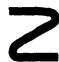
\includegraphics[keepaspectratio]{images/part001_58cd264b.jpg}}

应当注意，空间 \(\mathcal{M}(\mathrm{X};\mathbf{C})\) （或 \(\mathcal{M}(\mathrm{X};\mathbf{R})\) ）本身对淡一致结构不必是完备的（TVS, II, §6, No. 7）。

推论. --- 若 A 与 B 是 \(\mathcal{M}_{+}(\mathrm{X})\) 的两个淡闭子集，则 \(A + B\) 在 \(\mathcal{M}_{+}(\mathrm{X})\) 中淡闭（从而在 \(\mathcal{M}(\mathrm{X};\mathbf{C})\) 中也淡闭）。

这实际上是局部凸空间中弱完备的带顶点凸锥的一个一般性质（TVS, II, §6, No. 8, Prop. 11 的推论 2）。

命题 15. --- 设 H 为 \(\mathcal{M}(\mathrm{X};\mathbf{C})\) 的一个子集。下列性质等价：

\begin{enumerate}
\def\labelenumi{\alph{enumi})}
\item
  H 是淡有界的。
\item
  H 是淡相对紧的。
\item
  H 是等度连续的。
\item
  对 X 的每个紧子集 K，存在数 \(M_{K} \geqslant 0\)，使 \(|\mu(f)| \leqslant M_{K}\|f\|\) 对每个测度 \(\mu \in H\) 和每个函数 \(f \in \mathcal{K}(X, K; \mathbf{C})\) 成立。
\end{enumerate}

由于 \(\mathcal{K}(\mathrm{X};\mathbf{C})\) 是桶式空间（No. 1, Prop. 2），性质 a)、b) 与 c) 的等价性由 TVS, III, §4, No. 1 的 Scholium 得出。

显然 d) 蕴含 a)。最后，若 H 等度连续，则测度 \(\mu\in H\) 在 \(\mathcal{K}(X,K;\mathbf{C})\) 上的限制所成的集合也等度连续，由此得到条件 d)，因为 \(\mathcal{K}(X,K;\mathbf{C})\) 是赋范空间。

* 我们将在第 IV 章 §4 No. 6 中看到，命题 15 的诸条件也等价于如下条件：对 X 的每个紧子集 K，存在常数 \(\mathrm{M}_{\mathrm{K}}\)，使 \(|\mu|(\mathrm{K}) \leqslant \mathrm{M}_{\mathrm{K}}\) 对每个测度 \(\mu \in \mathrm{H}\) 成立。

推论 1. --- 设 \(\nu\) 为 X 上的正测度；测度 \(\mu\) （满足 \(|\mu| \leqslant \nu\) 的那些）所成的集合是淡紧的。

推论 2. --- 测度 \(\mu\) （满足 \(\|\mu\| \leqslant a\) ，其中 a 为任意有限数 \(>0\) ）所成的集合是淡紧的。

推论 3. --- 若 X 是紧的，则 X 上的正测度 \(\mu\) （满足 \(\|\mu\| = 1\) 的那些）所成的集合是淡紧的。

事实上，它是使 \(\|\mu\|\leqslant1\) 的测度所成的淡紧集（推论 2）与分别由关系式 \(\mu\geqslant0\) 和 \(\mu(1)=1\) 所确定的淡闭集的交（No. 8, Prop. 10 的推论 2）。

推论 4. --- 在空间 \(\mathcal{M}(\mathrm{X};\mathbf{C})\) 中，映射 \(\mu \mapsto \| \mu \|\) 对淡拓扑是下半连续的。

这是推论 2 的直接结果。

\pandocbounded{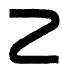
\includegraphics[keepaspectratio]{images/part001_13b41992.jpg}}

应当注意，映射 \(\mu \mapsto |\mu|\) （\(\mathcal{M}(\mathrm{X};\mathbf{C})\) 到自身的映射）对淡拓扑不必是连续的（习题 9）。

命题 16. --- 设 K 为 X 的紧子集，H 为 \(\mathcal{M}(\mathrm{X};\mathbf{C})\) 的淡有界子集；则双线性型 \((f,\mu)\mapsto\langle f,\mu\rangle\) 在 \(\mathcal{K}(\mathrm{X},\mathrm{K};\mathbf{C})\times\mathrm{H}\) 上连续，这里 \(\mathcal{K}(\mathrm{X},\mathrm{K};\mathbf{C})\) 装备一致收敛拓扑，而 H 装备淡拓扑。

事实上，存在数 \(M \geqslant 0\)，使得

\[
| \mu (f) | \leqslant \mathrm{M} \| f \|
\]

对每个函数 \(f \in \mathcal{K}(\mathrm{X},\mathrm{K};\mathbf{C})\) 和每个测度 \(\mu \in \mathrm{H}\) 成立（命题 15）。若 \(\mu_0\) 与 \(\mu\) 是属于 \(\mathrm{H}\) 的两个测度，\(f_0\) 与 \(f\) 是 \(\mathcal{K}(\mathrm{X},\mathrm{K};\mathbf{C})\) 中的两个函数，则

\[
\begin{array}{r l} | \mu (f) - \mu_ {0} (f _ {0}) | & = | \mu (f - f _ {0}) + \mu (f _ {0}) - \mu_ {0} (f _ {0}) | \\ & \leqslant \mathrm{M} \| f - f _ {0} \| + | \mu (f _ {0}) - \mu_ {0} (f _ {0}) |, \end{array}
\]

而当 \(\|f-f_{0}\|\) 与 \(|\mu(f_{0})-\mu_{0}(f_{0})|\) 任意小时，最后一个量也任意小，这就证明了命题。
